%%%%%%%%%%%%%%%%%%%%%% file typeinst.tex %%%%%%%%%%%%%%%%%%%%%%%%%
%
% This is the LaTeX source for the instructions to authors using
% the LaTeX document class 'llncs.cls' for contributions to
% the Lecture Notes in Computer Sciences series.
% http://www.springer.com/lncs       Springer Heidelberg 2006/05/04
%
% It may be used as a template for your own input - copy it
% to a new file with a new name and use it as the basis
% for your article.
%
% NB: the document class 'llncs' has its own and detailed documentation, see
% ftp://ftp.springer.de/data/pubftp/pub/tex/latex/llncs/latex2e/llncsdoc.pdf
%
%%%%%%%%%%%%%%%%%%%%%%%%%%%%%%%%%%%%%%%%%%%%%%%%%%%%%%%%%%%%%%%%%%%
\documentclass[runningheads,a4paper]{llncs}

%%%%%%%%%%%%%%%%%%%%%%%%%%%%

\usepackage[nodisplayskipstretch]{setspace}

%\setlength{\floatsep}{5pt}
\setlength{\textfloatsep}{14pt}

%\usepackage[
%  subtle
%  %moderate
%]{savetrees}
%------

%\usepackage{times}

%\linespread{0.97}



%\addtolength{\textfloatsep}{-0.4cm}

%\addtolength{\intextsep}{-0.3cm}

%----

%\setlength{\textfloatsep}{5pt} % Space between text and top/bottom floats
%\setlength{\floatsep}{5pt}     % Space between two consecutive floats

%\setlength{\intextsep}{5pt}    % Space above and below an in-text float

%\setlength{\textfloatsep}{7pt}

%\addtolength{\floatsep}{-0.5em}

% ROMOVE THIS IF YOU HAVE EXTRA SPACE.
\usepackage[font=small,skip=3pt]{caption}

%\captionsetup[figure]{skip=-2pt}

%\usepackage{titling}
%\setlength{\droptitle}{-3cm}

%\usepackage{dutchcal}

%\usepackage{dutchcal}

%\usepackage{pzccal}

%\usepackage[cal=boondox]{mathalfa}

\DeclareMathAlphabet{\mathpzc}{OT1}{pzc}{m}{it}

\usepackage[shortlabels]{enumitem}

\usepackage{subfiles}

\usepackage{tabularx}

\usepackage{adjustbox}

\usepackage{asymptote}

\usepackage{rotating}
%\usepackage{caption}
\usepackage[T1]{fontenc}
\usepackage{amssymb}
\usepackage{amsmath}
\usepackage{bm}
\setcounter{tocdepth}{3}
\usepackage{graphicx}
\usepackage{bussproofs}
\usepackage{supertabular}
\usepackage{longtable}
\usepackage{url}
\usepackage{afterpage}
\usepackage{tikz}
\usetikzlibrary{arrows}
\usetikzlibrary{decorations.pathmorphing}
\afterpage{\clearpage}
%\newtheorem{definition}{Definition}
%\newtheorem{proof}{Proof}
%\newproof{proof}{Proof}
%\newtheorem{mydef}{Definition}
%\newtheorem{myexample}{Example}
%\newtheorem{mytheorem}{Theorem}
%\newtheorem{mycorollary}{Corollary}
%\newtheorem{myobservation}{Observation}
%\newtheorem{mylemma}{Lemma}
\newtheorem{conj}{Conjecture}
%\newtheorem{inv}{Invariant}

\newtheorem{obs}{Observation}
%\newtheorem{proofoutline}{Proof outline}
%\newtheorem{myproof}{Proof of Proposition}
%\newtheorem{myproposition}{Proposition}
%\newtheorem{mylemma}{Lemma}
%\newtheorem{lemmaproof}{Proof of Lemma}
%\newtheorem{conjecture}{Conjecture}

%proof\_latex\_notheorem = [``proof'']

%\usepackage{amsthm}

%\usepackage{ntheorem}

\usepackage[lined,ruled,vlined,commentsnumbered]{algorithm2e}

%\usepackage{enumitem}

\usepackage{pbox}

\usepackage{stmaryrd}

\usepackage{varwidth}
\usepackage{booktabs}

\usepackage[mathscr]{euscript}

\usepackage{cancel}

\newcommand*{\Set}[2]{\ensuremath{\{#1\;|\;#2\}}}
\newcommand*{\Var}[1]{\ensuremath{\mathit{#1}}}
\newcommand*{\VarB}[1]{\ensuremath{\bm{\mathit{#1}}}}
\newcommand*{\VarCal}[1]{\ensuremath{\mathit{{\cal #1}}}}  % ditto in cal type

% Semantics of
\newcommand*{\Sem}[1]{\ensuremath{\llbracket #1 \rrbracket}}

% References to section, figure etc.
\newcommand*{\Sec}[1]{Sec.~\ref{#1}}
\newcommand*{\Fig}[2][]{Fig.~\ref{#2}{#1}}
\newcommand*{\Page}[1]{p.~\pageref{#1}}
\newcommand*{\Def}[1]{Definition~\ref{#1}}
\newcommand*{\Obs}[1]{Observation~\ref{#1}}
\newcommand*{\Alg}[1]{Algorithm~\ref{#1}}
\newcommand*{\Theorem}[1]{Theorem~\ref{#1}}
\newcommand*{\Lem}[1]{Lemma~\ref{#1}}
\newcommand*{\Conjecture}[1]{Conjecture~\ref{#1}}
\newcommand*{\Pt}[1]{pt.~\ref{#1}}
\newcommand*{\Ex}[1]{Example~\ref{#1}}

\newcommand*{\ESeq}[1]{\ensuremath{\Var{eseq}(#1)}}
\newcommand*{\TSeq}[1]{\ensuremath{\Var{tseq}(#1)}}

% Elements of a scenario
\newcommand*{\E}{\ensuremath{\mathcal{E}}}
\newcommand*{\C}{\ensuremath{\mathcal{C}}}

\newcommand*{\Clocks}{\ensuremath{\mathcal{C}}}   % The set of new clocks
\newcommand*{\U}{\ensuremath{\mathcal{U}}}


% t_ij, without and with behaviour
\newcommand*{\T}[2]{\ensuremath{t_{#1#2}}}
\newcommand*{\TB}[3]{\ensuremath{\T{#1}{#2}^{#3}}}
% tau_ij, symbolic and concrete
\newcommand*{\TT}[2]{\ensuremath{\tau_{#1,#2}}}
\newcommand*{\TTC}[2]{\ensuremath{\tau_{#1,#2}}}

% m_ij and M_ij, without and with scenario
\newcommand*{\Min}[2]{\ensuremath{m_{#1 #2}}}
\newcommand*{\MinB}[2]{\ensuremath{\bm{m}_{#1 #2}}}
\newcommand*{\Max}[2]{\ensuremath{M_{#1 #2}}}
\newcommand*{\MaxB}[2]{\ensuremath{\bm{M}_{#1 #2}}}
\newcommand*{\MinS}[3]{\ensuremath{\Min{#1}{#2}^{#3}}}
\newcommand*{\MinSB}[3]{\ensuremath{\MinB{#1}{#2}^{#3}}}
\newcommand*{\MaxS}[3]{\ensuremath{\Max{#1}{#2}^{#3}}}
\newcommand*{\MaxSB}[3]{\ensuremath{\MaxB{#1}{#2}^{#3}}}
% The interval in entry #2 #1 of a stable distance table for scenario #1
\newcommand*{\I}[3]{\ensuremath{\Var{I}^{#1}_{#2 #3}}}
\newcommand*{\IB}[3]{\ensuremath{\VarB{I}^{#1}_{#2 #3}}}
\newcommand*{\II}[2]{\ensuremath{\Var{I}_{#1 #2}}}
\newcommand*{\IIB}[2]{\ensuremath{\VarB{I}_{#1 #2}}}

% The min and max in a distance table
\newcommand*{\MinDT}[2]{\ensuremath{\underline{m}_{#1#2}}}
\newcommand*{\MaxDT}[2]{\ensuremath{\overline{M}_{#1#2}}}

% A distance table, without and with scenario
\newcommand*{\DTable}{\ensuremath{\mathcal{D}}}
\newcommand*{\DTableB}{\ensuremath{\bm{D}}}
\newcommand*{\DTableS}[1]{\ensuremath{\DTable^{#1}}}
\newcommand*{\DTableSB}[1]{\ensuremath{\DTableB^{#1}}}
% Ditto, with indices
\newcommand*{\DTS}[3]{\ensuremath{\DTableS{#1}[#2,#3]}}
% DTableS, stable version
\newcommand*{\DTableStable}[1]{\ensuremath{\DTableS{#1}_s}}
\newcommand*{\DTableStableB}[1]{\ensuremath{\DTableSB{#1}_s}}
% Ditto, with indices
\newcommand*{\DTSS}[3]{\ensuremath{\DTableStable{#1}[#2,#3]}}
\newcommand*{\DTset}[1]{\ensuremath{\DTableSB{#1}_{sync}}}
\newcommand*{\DTableSync}[1]{\ensuremath{\DTableS{#1}_{sync}}}
\newcommand*{\Dset}[1]{\ensuremath{\DTableSB{#1}_s}}

% Low and High elements of a pair in a distance table
\newcommand*{\Low}[2]{\ensuremath{l_{#1#2}}}
\newcommand*{\High}[2]{\ensuremath{h_{#1#2}}}

\newcommand*{\LowS}[3]{\ensuremath{l^{#3}_{#1#2}}}
\newcommand*{\HighS}[3]{\ensuremath{h^{#3}_{#1#2}}}

\newcommand*{\Table}[1]{\ensuremath{{\cal T}_{#1}}}

%\newcommand*{\Merge}{\ensuremath{\overset{z}{\cup}}}
\newcommand*{\Merge}{\ensuremath{\Cup}}

\newcommand*{\Z}{\ensuremath{\cal Z}}
\newcommand*{\BZ}{\ensuremath{\Behaviour{B}^z}}

\newcommand*{\Eq}[1]{\ensuremath{\VarCal{EQ}({#1})}}
%\newcommand*{\EqTA}[1]{\ensuremath{\mathit{Eq}({#1})}}
\newcommand*{\EqTA}{\ensuremath{\VarCal{EQT\!A}}}
\newcommand*{\Zpair}{\textit{z\_pair}}
\newcommand*{\J}{\ensuremath{\VarCal{J}}}
%%%%%%%%%%%%%%%%%%%%%%%%%%%%%%%%%%%%%
%%%%%%%%%%%%%%%%%%%%%%%%%%%%%%%%%%%%%
%%%%%%%%%%%%% N E D A %%%%%%%%%%%%%%%%%%%

\newcommand*{\GPath}{\ensuremath{\text{g-path}}}
\newcommand*{\Ftree}{\textit{f\_tree}}
\newcommand*{\Ftrees}{\textit{f\_trees}}


\newcommand*{\Modes}{\ensuremath{\mathcal{M}^{\mu_0}_{\mu_F}}}

\newcommand*{\Mi}{\ensuremath{\mu^{i}}}
\newcommand*{\Mf}{\ensuremath{\mu^{f}}}

\newcommand*{\MiS}[1]{\ensuremath{\mu^{i}_{#1}}}
\newcommand*{\MfS}[1]{\ensuremath{\mu^{f}_{#1}}}

\newcommand*{\Initial}[1]{\ensuremath{\Var{imode}(#1)}}
\newcommand*{\Final}[1]{\ensuremath{\Var{fmode}(#1)}}

\newcommand*{\Comp}[1]{\ensuremath{\mathit{Comp}({#1})}}

\newcommand*{\Composed}[1]{\ensuremath{\mathit{Composed}({#1})}}

\newcommand*{\Cons}[1]{\ensuremath{\mathit{Cons}({#1})}}

\newcommand*{\STA}[1]{\ensuremath{\VarCal{T\!A}(#1)}}

\newcommand*{\ATA}{\ensuremath{\VarCal{T\!A}}}


\newcommand*{\STOC}[1]{\ensuremath{\VarCal{A}^{#1}}}

\newcommand*{\SOC}[1]{\ensuremath{\VarCal{A}^{#1}_{a}}}

\newcommand*{\M}{\ensuremath{\mathcal{M}}}

\newcommand*{\Lab}{\ensuremath{\mathcal{L}}}
\newcommand*{\LL}{\ensuremath{\mathcal{L}_l}}
\newcommand*{\LM}{\ensuremath{\mathcal{L}_\M}}
\newcommand*{\None}{\ensuremath{\mathit{none}}}

\newcommand*{\Tree}[1]{\ensuremath{\mathcal{T}^{#1}}}

%\newcommand*{\Graph}[1]{\ensuremath{\mathcal{G}^{#1}}}

%\newcommand*{\Pruned}{\ensuremath{\mathcal{T}^{\Xi}_{p}}}

\newcommand*{\PrunedTree}[1]{\ensuremath{\mathcal{T}^{#1}_{p}}}

\newcommand*{\ConsTree}[1]{\ensuremath{\mathcal{T}^{#1}_{c}}}

\newcommand*{\OptTree}[1]{\ensuremath{\mathcal{T}^{#1}_{o}}}

\newcommand*{\DisTree}[1]{\ensuremath{\mathcal{T}^{#1}_{d}}}

\newcommand*{\AllocTree}[1]{\ensuremath{\mathcal{T}^{#1}_{a}}}

\newcommand*{\Lang}[1]{\ensuremath{L(#1)}}

%\newcommand*{\MapV}{\ensuremath{M_V}}

\newcommand*{\MapV}{\ensuremath{\mathit{VM}}}

\newcommand*{\MapVprime}{\ensuremath{M'_V}}

\newcommand*{\LabV}{\ensuremath{B_V}}

\newcommand*{\LabR}{\ensuremath{B_R}}

\newcommand*{\STP}{\ensuremath{\mathcal{S}(\mathcal{T}^{\Xi})}}

\newcommand*{\STC}{\ensuremath{\mathcal{S}(\mathcal{T}^{\Xi}_c)}}

\newcommand*{\CP}[1]{\ensuremath{\VarCal{S}(\mathcal{T}^{\Xi}_{#1})}}



% For transitions
\newcommand*{\Source}[1]{\ensuremath{\Var{source}(#1)}}
\newcommand*{\Target}[1]{\ensuremath{\Var{target}(#1)}}

\newcommand*{\Label}[1]{\ensuremath{\Var{label}(#1)}}
\newcommand*{\Event}[1]{\ensuremath{\Var{event}(#1)}}
\newcommand*{\Events}[1]{\ensuremath{\Var{events}(#1)}}
\newcommand*{\Constraints}[1]{\ensuremath{\Var{constraints}(#1)}}

% For paths
\newcommand*{\Or}[1]{\ensuremath{\Var{origin}(#1)}}
\newcommand*{\End}[1]{\ensuremath{\Var{end}(#1)}}

% For nodes
\newcommand*{\Out}[1]{\ensuremath{\Var{out}(#1)}}
\newcommand*{\In}[1]{\ensuremath{\Var{in}(#1)}}

%\newcommand*{\Assign}[1]{\ensuremath{\Var{assign}}}

%\newcommand*{\Alloc}{\Var{alloc}}

\newcommand*{\Alloc}[1]{\ensuremath{\Var{alloc}_{#1}}}

\newcommand*{\Cost}{\Var{cost}}

\newcommand*{\Ext}[1]{\ensuremath{\Var{ext}(#1)}}

\newcommand*{\CostTree}{\Var{cost\_tree}}

\newcommand*{\AllocPath}[1]{\ensuremath{\Var{alloc}_{#1}}}

\newcommand*{\CostPath}{\ensuremath{\Var{cost\_path}}}

\newcommand*{\ComputeCost}{\ensuremath{\Var{compute\_cost}}}

\newcommand*{\NestedIn}{\Var{nested\_in}}

\newcommand*{\VLeaves}{\Var{visitedLL}}

\newcommand*{\VAnc}{\Var{inCycles}}


\newcommand*{\Assoc}{\Var{assoc}}
\newcommand*{\TempAssoc}{\Var{newAssoc}}
\newcommand*{\Pool}{\Var{pool}}
\newcommand*{\TempPool}{\Var{newPool}}

\newcommand*{\NLA}{\Var{NLA}}

\newcommand*{\CR}{\Var{CR}}

\newcommand*{\Forks}{\Var{forks}}

\newcommand*{\RNeeded}{\Var{really\_needed}}

\newcommand*{\OldNeeded}{\Var{old\_\Needed}}

\newcommand*{\LabN}{\ensuremath{\mathit{\Lab_{n}}}}

\newcommand*{\Ranges}{\Var{ranges}}

\newcommand*{\ConfRanges}{\Var{conf\_ranges}}

\newcommand*{\PathClocks}{path\_clocks}

\newcommand*{\Active}{\Var{Active}}

\newcommand*{\Alive}{\Var{alive}}

\newcommand*{\LastRef}{\Var{last\_ref}}

\newcommand*{\Weight}{\Var{weight}}

%\newcommand*{\Disj}[1]{\ensuremath{\mathcal{P}^{#1}_{d}}}

\newcommand*{\Paths}[1]{\ensuremath{\mathcal{P}({#1})}}

\newcommand*{\Disj}[1]{\ensuremath{\mathcal{P}_{d}({#1})}}


\newcommand*{\Used}{\Var{used}}
\newcommand*{\Born}{\Var{born}}

\newcommand*{\ActTarget}{\Var{act\_target}}

\newcommand*{\Needed}{\Var{needed}}

\newcommand*{\RealCost}{\Var{real\_cost}}

\newcommand*{\OptimalCost}{\Var{opt\_cost}}

\newcommand*{\Range}{\Var{range}}

\newcommand*{\Tr}{\Var{transitions}}

\newcommand*{\Conflict}{\Var{conflict}}

\newcommand*{\InRanges}{\Var{In\_Ranges}}
%%%%%%%%%%%%%%%%%%%%%%%%%%%%%%%%%%%%%


\newcommand*{\ClockRef}{\Var{clock\_ref}}

\newcommand*{\AbsSynt}{\Var{AbsSynt}}
\newcommand*{\Abstract}[1]{\ensuremath{\AbsSynt(#1)}}
\newcommand*{\Abs}{\Var{Abs}}

%\newcommand*{\STA}[1]{\ensuremath{\VarCal{T\!A}(#1)}}
%%%%%%%%%%%%%%%%%%%%%%%%%%%%%%%%%%%%%

\newcommand*{\Cprime}{\ensuremath{\mathcal{C}^\prime}}

\newcommand*{\DImplies}{\ensuremath{\leadsto}}
\newcommand*{\Implies}{\ensuremath{\DImplies^+}}

\newcommand*{\Dcyclic}{\ensuremath{\leftrightarrow}}

\newcommand*{\Cyclic}{\ensuremath{\overset{+}{\Dcyclic}}}

\newcommand*{\DImp}[1]{\ensuremath{\DImplies #1}}

%\newcommand*{\CycSupp}[2]{\ensuremath{S_{#1}^{\DImp{#2}}}}

\newcommand*{\CycSupp}[2]{\ensuremath{S_{#1}^{\triangleright{#2}}}}

\newcommand*{\DepName}{\ensuremath{\rightarrow}}
\newcommand*{\Dep}[2]{\ensuremath{#1 \DepName #2}}
\newcommand*{\NotDep}[2]{\ensuremath{#1 \not\DepName #2}}

\newcommand*{\LessThan}{\ensuremath{\preceq}}


 % the data structures
\newcommand*{\CS}{\textit{C}}
\newcommand*{\WS}{\textit{WS}}
%\newcommand*{\CD}{\textit{CD}}
\newcommand*{\ICD}{\textit{ICD}}
\newcommand*{\CyDep}{\textit{CyDep}}
\newcommand*{\LS}{\textit{L}}

\newcommand*{\CDTableStable}[1]{\ensuremath{\mathcal{C}(\DTableStable{#1})}}

\newcommand*{\CDNETableStable}[1]{\ensuremath{\mathcal{C}(\DTableStable{#1})^{>,<}}}

\newcommand*{\DSup}{\ensuremath{\Var{DSupp}}}

\newcommand*{\A}[1]{\ensuremath{\mathcal{A}_{#1}}}

\newcommand*{\Anc}[1]{\ensuremath{\mathit{Anch}_{#1}}}

%%%%%%%%%%%%%%%%%%%%%%%%%%%%%%%%%%%%%
\newcommand*{\DScenario}{\ensuremath{\Xi}}
\newcommand*{\Dist}[1]{\ensuremath{dstr}_{#1}}
\newcommand*{\Par}{\ensuremath{\preccurlyeq}}
\newcommand*{\ParS}[1]{\ensuremath{\prec}_{#1}}
\newcommand*{\ParSE}[1]{\ensuremath{\prec}_{#1}^{x}}
\newcommand*{\ParSA}[1]{\ensuremath{\prec}_{#1}^{e}}
\newcommand*{\TotalS}[1]{\ensuremath{<}_{#1}}
\newcommand*{\ESet}[1]{\ensuremath{\Var{eset}(#1)}}
\newcommand*{\Dash}{`{\bf -}'}
\newcommand*{\DashMath}{\textrm{\bf -}}
\newcommand*{\Sim}[1]{\ensuremath{Sim}_{#1}}
\newcommand*{\SimClass}[1]{\ensuremath{SimClass}_{#1}}
\newcommand*{\SyncSet}{\ensuremath{SyncSet}}
\newcommand*{\DR}[1]{\ensuremath{\mathcal{DR}_{#1}}}
\newcommand*{\Can}[1]{\ensuremath{\mathit{C}}_{#1}}
\newcommand*{\PR}[1]{\ensuremath{\ParS{#1}}}
\newcommand*{\DRS}[1]{\ensuremath{\mathcal{DR}_{#1}^s}}
\newcommand*{\DRE}[1]{\ensuremath{\mathcal{DR}_{#1}^x}}
\newcommand*{\DRSE}[1]{\ensuremath{\mathcal{DR}_{#1}^{xs}}}
\newcommand*{\DF}[1]{\ensuremath{\mathcal{DF}_{#1}}}
\newcommand*{\DFS}[1]{\ensuremath{\mathcal{DF}_{#1}^{s}}}
\newcommand*{\DFE}[1]{\ensuremath{\mathcal{DF}_{#1}^{xs}}}
\newcommand*{\DFEX}[1]{\ensuremath{\mathcal{DF}_{#1}^{x}}}
\newcommand*{\Proj}[1]{\ensuremath{\mathcal{P}_{#1}}}
\newcommand*{\SeqS}{\ensuremath{\mathit{s}}}
\newcommand*{\SeqSC}{\ensuremath{\mathit{sc}}}
\newcommand{\precdot}{\prec\mathrel{\mkern-5mu}\mathrel{\cdot}}
\newcommand*{\ParSdot}[1]{\ensuremath{\precdot}_{#1}}
\newcommand*{\ParScover}[1]{\ensuremath{\prec}_{#1}^{c}}
\newcommand*{\Perm}[1]{\ensuremath{perm}(#1)}
\newcommand*{\K}[2]{\ensuremath{d}_K(#1,#2)}
\newcommand*{\RK}[1]{\ensuremath{r}_K(#1)}
\newcommand*{\CK}[1]{\ensuremath{r}_c(#1)}
%\newcommand*{\CD}[3]{\ensuremath{{{d}_c}^{#3}(#1,#2)}}
\newcommand*{\CD}[2]{\ensuremath{{{d}_c}(#1,#2)}}
\newcommand*{\DDist}{\ensuremath{\Var{d-distance}}}
\newcommand*{\CDiff}{\textit{c\_diff}}
%\newcommand*{\CDis}{\textit{c\_dis}}
\newcommand*{\CDis}[1]{\ensuremath{{dsg}_{#1}}}
\newcommand*{\CBD}[1]{\ensuremath{{cbd}_{#1}}}
\newcommand*{\OBD}[1]{\ensuremath{{obd}_{#1}}}
\newcommand*{\BAR}{\ensuremath{\boldsymbol{|}}}
\newcommand*{\D}{\ensuremath{\mathcal{D}}}
%%%%%%%%%%%%%%%%%%%%%%%%%%%%%%%%%%%%%


\newcommand*{\Univ}{\ensuremath{B_{\xi}}}

%\newcommand*{\AbsTime}{\Var{AbsTime}}
%\newcommand*{\Abs}[1]{\ensuremath{\AbsTime(#1)}}

\newcommand*{\MinValue}[1]{\ensuremath{min\_value(#1)}}
\newcommand*{\MaxValue}[1]{\ensuremath{max\_value(#1)}}

\newcommand*{\IsCovered}[3]{\ensuremath{is\_covered(#1, #2, #3)}}

\newcommand*{\OurClass}{\ensuremath{\mathit{TA_{DS}}}}
\newcommand*{\SynthClass}{\ensuremath{\mathit{TA_{synth}}}}

\newcommand*{\Unseen}{\Var{Unseen}}
\newcommand*{\Seen}{\Var{Seen}}

% Transition j on path p_{\xi}
\newcommand*{\tr}[2]{\ensuremath{r_{#1}^{#2}}}
%\newcommand*{\tr}[2]{\ensuremath{tr(#1,p_{#2})}}



\newcommand*{\Beginat}{\Var{Begin\_at}}

\newcommand*{\MG}{\VarCal{M}}             % The symbol for a  mode grap
\newcommand*{\TA}{\VarCal{A}}             % and for the constructed automaton
\newcommand*{\Legal}{\ensuremath{B_{\MG}}} % The set of legal behaviours for MG
\newcommand*{\Allowed}[1]{\ensuremath{\Var{Allowed}(#1)}}

%\newcommand*{\Sup}[1]{\ensuremath{\Var{Supp}(#1)}}
%\newcommand*{\Sup}{\ensuremath{\Var{Supp}}}

\newcommand*{\Sup}[1]{\ensuremath{\Var{Supp}(#1)}}


\newcommand*{\Behaviour}[1]{\ensuremath{\mathcal{#1}}}

\newcommand{\ParaTitle}[1]{\noindent\textbf{#1.}}


\newcommand*{\Ind}{\hspace{1em}}
\newcommand*{\ind}{\hspace{0.5em}}


\usepackage{url}
\urldef{\mailsa}\path|{alfred.hofmann, ursula.barth, ingrid.haas,
  frank.holzwarth,|
\urldef{\mailsb}\path|anna.kramer, leonie.kunz, christine.reiss, nicole.sator,|
\urldef{\mailsc}\path|erika.siebert-cole, peter.strasser, lncs}@springer.com|
\newcommand{\keywords}[1]{\par\addvspace\baselineskip
  \noindent\keywordname\enspace\ignorespaces#1}

%%%%%%%%%%

\begin{document}

\mainmatter  % start of an individual contribution

% first the title is needed
\title{Timed Scenario Expressions and Realisability}

% a short form should be given in case it is too long for the running head
\titlerunning{Timed Scenario Expressions and Realisability}

\author{Neda Saeedloei\inst{*} \and Feliks Klu\'{z}niak}
%\author{Neda Saeedloei}
%\affil{Towson University}
%
\authorrunning{Neda Saeedloei and Feliks Klu\'{z}niak}
% abbreviated author list (for running head)
%
%%%% list of authors for the TOC (use if author list has to be modified)
\tocauthor{Neda Saeedloei, Feliks Klu\'{z}niak}
%
%\institute{Towson University\\
%\email{nsaeedloei@towson.edu}

%\author{Neda Saeedloei\inst{1} \and Feliks Klu\'{z}niak\inst{2}}
%\author{Neda Saeedloei}
%
%\authorrunning{Neda Saeedloei and Feliks  Klu\'{z}niak}
%\authorrunning{Neda Saeedloei}
% abbreviated author list (for running head)
%
%%%% list of authors for the TOC (use if author list has to be modified)
%\tocauthor{Neda Saeedloei, Feliks Klu\'{z}niak}
%\tocauthor{Neda Saeedloei}
%
\institute{* Towson University\\
  \email{nsaeedloei@towson.edu}
%  ,
%\and
%RelationalAI\\
%\email{feliks.kluzniak@relational.ai}
}

\toctitle{Timed Scenario Expressions and Realisability}
\tocauthor{Authors' Instructions}
\maketitle

% Without this the first footnote will have number 3, since there are footnotes
% in the title.
\setcounter{footnote}{0}

%\vspace{-1.6em}
\begin{abstract}
  We introduce expressions formed from distributed timed scenario.
  Such expressions allow us to specify complex distributed behaviours in a
  hierarchical fashion.
We define the semantics and consistency of a scenario
expression. We then address the problem of realisability of sets
of sequential timed scenarios as scenario expressions and
present an efficient algorithm which produces a non-trivial scenario
expression that preserves the semantics of the original set of
scenarios. Our method directly handles explicit time constraints
and produces a scenario expression whose time constraints are
inferred from those of the realised set.
\end{abstract}
%%%%%%%%%%%%%%%%%%%%%%%%%%%%%%%%%%%%%%%%%%%%%%%%%%%%%
%\vspace{-2em}
\section{Introduction}
\label{sec-intro}
The problem of realisability of global models, e.g., global (session)
types \cite{BEJLERI-2009,Castagna-2011,Honda-2016,Hans-2016}, global
choreographies \cite{Franco-2022}, global labelled transition
systems \cite{Beek-2023} and global languages
has attracted many researchers over the past several years.
A realisation of a global model is a set of
collaborating computing entities which
are executed concurrently, and whose behaviours, obtained from their
(synchronous or asynchronous) interactions, are exactly those that are
obtained from the global models.
For example, a global model can be the parallel composition of a set
of labelled transition systems, each of which models the local
behaviour of a component.
An interesting, but challenging question is how to determine whether a
global model is realisable and, if so, how to obtain a realisation.

We are interested in the problem of realisability for global
models that take the form of sets of sequential timed
scenarios. Given such a set, our goal is to
obtain a \emph{timed scenario expression} that realises the set.

In earlier work we developed the notions of sequential
timed scenarios (scenarios for short) \cite{neda-2018-2} and
distributed timed scenarios \cite{DTS-2025}.
A scenario is a sequence of (names of) events along with a set of
constraints on the times at which these events occur
(see \Sec{sec-seq} for more details).
A distributed timed scenario (DTS) is a collection of
components, each of which is a timed
scenario (see \Sec{sec-dts} for more details).
Each component performs its specified actions, represented as a
sequence of events, concurrently with
other components. Components can communicate or
synchronise with each other by performing the same action
simultaneously.
%The idea is that each component performs its specified
%actions, represented as a sequence of events, independently from
%other components. However, from time to
%time, the components communicate or synchronise with each other
%by performing the same action simultaneously.
A DTS, $\DScenario$, is viewed as a parallel composition of its components and its
semantics is defined as a set of distributed behaviours, i.e., the set
of all possible interleavings of events in the components of
$\DScenario$ that satisfy the constraints and the synchronising
requirements of $\DScenario$.

Given a set, $\mathcal{S}$, of scenarios over a set of events,
$\Sigma_{\mathcal{S}}$,
the stable distance relation \cite{DTS-2025} of $\mathcal{S}$
is $\DR{\mathcal{S}}=(\ParS{\mathcal{S}},\DF{\mathcal{S}})$.
The partial order $\ParS{\mathcal{S}}$
captures all the ordering dependencies between events in
$\mathcal{S}$, while the distance function, $\DF{\mathcal{S}}$,
expresses constraints on the time between
every pair of events $e$ and $e'$,
where $e\ParS{\mathcal{S}}e'$. A projection of
$\DR{\mathcal{S}}$ is a scenario over $\Sigma_{\mathcal{S}}$ whose
sequence of events agrees with
$\ParS{\mathcal{S}}$ and whose constraints satisfy
%includes the tightest constraints that satisfy
the constraints captured by $\DF{\mathcal{S}}$.

In the current paper we introduce \emph{timed scenario expressions}
and solve the problem of realisability of sets of
scenarios as scenario expressions.
%That is, given a global model of the behaviours of a system, captured
%by a set of scenarios, $\mathcal{S}$, we produce a scenario expression that expresses
%the same set of behaviours that are allowed by the members of $\mathcal{S}$.
So our contribution is twofold:
%\subsubsection{Contributions}
% \setlist{nolistsep}
%\begin{enumerate}[noitemsep]
%\item

First, we introduce a limited form of timed scenario expressions (expressions
for short), as a means
of constructing hierarchical models of complex systems, whose constituent
parts are distributed systems (\Sec{sec-exp}). Intuitively, an expression is built by
repeatedly applying three operators, namely choice,
concatenation and parallel composition (denoted by $\BAR$, $\circ$ and
$||$\footnote{We do not consider the Kleene star ($*$) operator here, as its
introduction opens up interesting questions that cannot
be addressed in the confines of the current paper.}, respectively), to
distributed scenarios. In its simplest form an
expression is just a single DTS.
Given an expression $E$, we
define its semantics, denoted by $\Sem{E}$, in terms of the set
of distributed behaviours that are expressed by $E$.
%\item

Second, we tackle the problem of realisability of sets of (sequential)
scenarios as expressions (\Sec{sec-realize}). Given a finite
set, $\mathcal{S}$, of scenarios, we produce a scenario
expression, $E$, that realises $\mathcal{S}$,
i.e., $\Sem{E}$ is identical to the union of the sets of behaviours
specified by the members of $\mathcal{S}$.

We identify two criteria for realisability of $\mathcal{S}$ as a
single DTS: $\mathcal{S}$ is realisable by a DTS iff (i) it
is \emph{order-closed}, and (ii) all its members are \emph{compatible}, in
terms of their constraints, with $\DR{\mathcal{S}}$.
Intuitively,
$\mathcal{S}$ is order-closed if, for every projection of
$\DR{\mathcal{S}}$, there is a scenario in $\mathcal{S}$
with that exact sequence of events, and vice versa.
A scenario $\SeqSC\in\mathcal{S}$ is compatible with
$\DR{\mathcal{S}}$ if its set of constraints is equivalent to the set
of constraints of the projection of $\DR{\mathcal{S}}$ that
has the same sequence of events as $\SeqSC$.

If $\mathcal{S}$ is not realisable by a single DTS,
then it must be divided into
partitions, in such a way that each partition is order-closed and all
its members are compatible with the distance relation of the
partition. Once every partition is realisable by a single DTS, the
resulting expression will be a choice between these
distributed scenarios.

The novelty of our work is primarily in the use of (stable) distance
relations \cite{DTS-2025} as a linchpin of an efficient method
%, confirmed by our experimental results,
for the realisation problem.
By identifying the necessary and sufficient conditions for the
realisability of a set of scenarios as a DTS, we address the problem
that was left open in our earlier work \cite{DTS-2025}.



%The reason we do not consider the Kleene star ($*$) operator in our
%expressions in the current paper is that they make the realisation
%problem significantly more complex.
%To fully address the problem of realisability where the
%resulting expressions involve $*$
%would require developing new apparatus and
%techniques (in addition to what is developed in the current paper),
%which could not be presented in the current paper due to
%the page limitation.
%\end{enumerate}
%\vspace{-1.4em}
\subsubsection{Related Work}
In our earlier work \cite{DTS-2025} we developed an algorithm for
solving the problem
of realisability of sets of (sequential) scenarios as distributed scenarios.
Given a set of scenarios, our algorithm determines whether
the set is realisable by a \emph{single} DTS, i.e.,
whether there is a DTS whose semantics is identical
to the union of the behaviours described by the members of
the set. If so, the algorithm produces such a DTS.
Despite some similarities, the problem that we tackle in the current
paper is fundamentally different.

%----------------------
The comparison of our sequential timed scenarios
with simple temporal networks (STNs) \cite{DECHTER1991}, as well as
with message sequence charts (MSCs) \cite{Harel2003,MSCs}, is presented
elsewhere \cite{DTS-2025}.
Similarities between
%our distance relations and timed partial
%orders (TPOs) of Watanabe et al. \cite{watanabe2023}, as well as
%between
the distributed behaviours of distributed timed scenarios and the
timed traces of Balaguer et al. \cite{hal-2012} are also discussed
in our earlier work \cite{DTS-2025}.

%The comparison of our stable distance tables with Difference Bounds
%Matrices is presented elsewhere \cite{neda-2017,neda-2018-2}.

The problem of realisability has been investigated in a variety of settings,
%of global models
%has been investigated
e.g., for message sequence
charts \cite{Alur-2003}, global session
types \cite{BEJLERI-2009,Castagna-2011,Honda-2016,Hans-2016},
pomsets \cite{GUANCIALE201969},
global labelled transition systems \cite{Beek-2023},
%more recently for
choreography languages \cite{Franco-2022} and team
automata \cite{Beek-2024}. Unlike in all
these works the realisability of our sets of sequential scenarios as
scenario expressions is
determined by precise time analysis enabled by our distance
relations.
%The distance relations enable us to reason about the underlying partail
%order, as well as the time constraints between various events in
%scenarios, both of which are essential for realisability of
That is, in our setting we are able to directly reason
about realisability of models that include explicit time constraints
and produce realisations that involve time constraints.


%----------------------------------
%\vspace{-1em}
%\section{Preliminaries}
%\label{sec-preliminaries}
%\vspace{-1em}
%-----------------------------------
%\subsection{Timed automata}
%\label{timed}
%\input{timed_automata-new}
%----------------------------------
%\vspace{-1em}
\section{Preliminaries}
\label{sec-prelim}
This section briefly recounts our
earlier work \cite{neda-2018-2,DTS-2025}.
%\vspace{-0.5em}
\subsection{Sequential Timed Scenarios}
\label{sec-seq}
Let $\Sigma$ be a finite set of symbols called \emph{events}.  A
\emph{behaviour}\footnote{The notion of ``behaviour'' is equivalent to
that of Alur's ``timed word'' \cite{alur94}.
%We found the term ``behaviour'' more suitable and intuitive in the
%context of timed scenarios.
}
over $\Sigma$ is a non-empty
  sequence $(e_0, t_0)(e_1, t_1)(e_2, t_2)\dots$ , such that
  $e_i \in \Sigma$, $t_i \in \mathbb{R}^{\geq
  0}$ and $t_{i-1}\leq t_i$ for $i \in \{1, 2 \dots\}$.
 For a finite behaviour $\Behaviour{B} = (e_0,t_0) (e_1,t_1) \ldots
(e_{n-1},t_{n-1})$ of length $n$ ($n \in \mathbb{N}^{>0}$), and for any $0 \leq i < j < n$,
  the \emph{distance}, in time units, of
event $j$ from event $i$ in $\Behaviour{B}$ is denoted by
$\T{i}{j}^\Behaviour{B}$.  That is,
$\T{i}{j}^\Behaviour{B} = t_j - t_i$.

A \emph{sequential timed scenario} (\emph{scenario} for short) of length
$n \in \mathbb{N}$ over $\Sigma$ is a pair $(\E, \C)$,
where $\E = e_o e_1 ... e_{n-1}$ is a non-empty sequence of events
from $\Sigma$, and
$\C \subset \Phi(n)$ is a finite set of constraints.
A constraint in $\Phi(n)$ is
  of the form $b \sim a$, where  $b$ is the symbol \TT{i}{j} (for some
  integers
     $0 \leq i < j < n$), $\sim\in\{\leq,\geq,=\}$\footnote{To keep the presentation compact, we do not allow sharp
    inequalities.
    %: allowing them would complicate our definitions,
    %without affecting the general principles.
    %Notice that    Sharp inequalities
    They are mostly of theoretical interest: in practice we can measure time only
    with some finite granularity $\gamma$, so $x < c$ is for all practical
    purposes equivalent to $x \leq c - \gamma$.}
    %To keep the presentation compact, we do not allow strict
    %inequalities \cite{neda-2018-2}.}
    and $a\in\mathbb{Q}$ is a constant.
The interpretation is that \TT{i}{j} is the time distance
between the $i$-th and the $j$-th events in the behaviours described
by a scenario.
% ARE DEFAULT CONSTRAINTS NECESSARY?
The constraints $\TT{i}{j} \geq 0$ and $\TT{i}{j} \leq \infty$
are called \emph{default constraints}.

We use $\Sigma_{\xi}= \{e_0, e_1, \dots, e_n \} \subseteq \Sigma$ to
denote the set of events in $\E$.

A behaviour $\Behaviour{B} =
(e_0,t_0)(e_1,t_1)\ldots(e_{n-1},t_{n-1})$ over $\Sigma$
is \emph{allowed} by scenario $\xi = (\E, \C)$ iff $ \E = e_0 \dots
e_{n-1}$ and every  $\TT{i}{j} \sim a$ in \C{} evaluates to true
after $\TT{i}{j}$ is replaced by \TB{i}{j}{\Behaviour{B}}.
The \emph{semantics} of scenario $\xi$, denoted by \Sem{\xi}, is the
set of behaviours that are allowed by $\xi$.
%NEDA: RESTORE IF NEEDED:
%Additionally, if $\mathcal{S}=\{\xi_1,\dots,\xi_n\}$ is a finite set of
%sequential scenarios, the semantics of $\mathcal{S}$ is
%$\Sem{\mathcal{S}} = \bigcup_{1\leq i \leq n} \Sem{\xi_i}$.
A scenario $\xi$ is \emph{consistent} iff $\Sem{\xi} \neq \emptyset$.

For example, $\xi = (a b c, \{ \TTC{0}{1} \geq
3, \TTC{0}{2} \leq 7\})$ is a consistent scenario:
$\Sem{\xi} =
\Set{(a,t_0)(b,t_1)(c,t_2)}{t_0 \leq t_1 \leq t_2
  \wedge t_1 - t_0 \geq 3
  \wedge t_2 - t_0 \leq 7}$.
%-----------------------------------------
% NEDA: Do we need equivalent in this paper?
%Two scenarios $\xi = (\E, \C_1)$ and $\eta = (\E, \C_2)$
%are \emph{equivalent} iff $\Sem{\xi} = \Sem{\eta}$. For example, $\gamma$
%and $\eta$ of \Fig{equality-rightleg} are equivalent.

%In the rest of the paper every time we write ``scenario'' without
%qualifications we mean sequential scenario.

%\vspace{-0.5em}
\subsection{Distributed Timed Scenarios}
\label{sec-dts}
The scenario $\xi=(\E,\C)$ is in \emph{normalised form} iff
every event of \E{} has only one occurrence in \E{}\footnote{
%An arbitrary scenario can be trivially transformed to normalized
%form.
If there is more than one event with the same name, say $a$, in a scenario
of length $n$, the $k$th ($1<k\leq n-1$) occurrence of
$a$ can be replaced with $a_{k}$.}.
%In the rest of the paper we assume all the sequential scenarios are
%normalized.
If $\xi$ is in normalised form, then each event is uniquely
identified by its name.
If event $i$ in $\xi$ is $a$, we will use $t_a$
(instead of $t_i$) to refer to the time of $a$ in a behaviour
$\Behaviour{B}\in \Sem{\xi}$. If event $j$ ($i<j$) in
$\xi$ is $b$, we will use $\TT{a}{b}$ (instead of \TT{i}{j}) in a
constraint that restricts the time distance between $a$ and $b$, and
$\T{a}{b}^\Behaviour{B}$ (instead of $\T{i}{j}^\Behaviour{B}$) to
represent the time distance between $a$ and $b$ in \Behaviour{B}.
%For a consistent and normalised scenario $\xi = (\E, \C)$ over
%$\Sigma$, where $\E = e_0 e_1 \dots e_n$, we use
%$\Sigma_{\xi}= \{e_0, e_1, \dots, e_n \} \subseteq \Sigma$ to denote
%the set of events in $\E$.
%We assume $\Sigma_{\xi}$ includes the event \Dash.
%We explain the motivation for this after \Def{def-sync-event}.
Naturally, the sequence $\E = e_o e_1 ... e_{n}$ of a normalised scenario $\xi$ induces a
total order on $\Sigma_{\xi}$. We use $\TotalS{\xi}$ to denote this
total order: for two events $e_i$ and $e_j$ in
$\E$, $e_i \TotalS{\xi} e_j \iff i < j$.

A \emph{distributed timed scenario} (\emph{DTS} or \emph{distributed
scenario} for short) over $\Sigma$ is a finite collection of
(sequential) scenarios, denoted by $\DScenario=\D(\xi_1,\dots,\xi_n)$,
such that each $\xi_j$ ($1\leq j \leq n$) is consistent and is in
normalised form.
We refer to each $\xi_j$ as a \emph{component of} \DScenario.
  We use $\Sigma_{\DScenario} = \Sigma_{\xi_1} \cup \dots \cup
  \Sigma_{\xi_n}\subseteq\Sigma$ to denote the set of events of \DScenario.
  We say \DScenario{} % over $\Sigma$ is
is \emph{well-formed} iff $\ParS{\DScenario}\subseteq \Sigma_{\DScenario} \times
\Sigma_{\DScenario}$, defined as the transitive closure of $\bigcup_{\xi \in \Xi}
\TotalS{\xi}$, is a strict partial order on $\Sigma_{\DScenario}$.

For $\Behaviour{B}$, a behaviour over $\Sigma$, and $\xi$, a
scenario, such that $\Sigma_{\xi} \subseteq \Sigma$,
the \emph{restriction} of \Behaviour{B} to $\xi$, denoted by
$\Behaviour{B}_{\xi}$, is the maximal subsequence of \Behaviour{B} such that
every event of $\Behaviour{B}_{\xi}$ is in $\Sigma_{\xi}$.
If $\DScenario=\D(\xi_1,\dots,\xi_n)$ is a DTS
over $\Sigma$, then behaviour \Behaviour{B} over
$\Sigma$ is
\emph{allowed} by \DScenario{} iff, for every component $\xi_i$ of \DScenario{}
($1\leq i\leq n$), $\Behaviour{B}_{\xi_i} \in \Sem{\xi_i}$.
Clearly, if \DScenario{} is not well-formed, then it allows no behaviours.
The \emph{semantics} of \DScenario,
denoted by \Sem{\DScenario}, is the set of behaviours that are allowed
by \DScenario.
A DTS \DScenario{} is \emph{consistent}
iff $\Sem{\DScenario} \neq \emptyset$.
%It is \emph{inconsistent} iff $\Sem{\DScenario}=\emptyset$.
% NEDA: IF WE NEED EQUIVALENCE< RESTORE.
%Two consistent distributed scenarios, $\DScenario$ and $\DScenario'$,
%over $\Sigma$, are \emph{equivalent} (denoted by $\DScenario \equiv
%\DScenario'$) iff $\Sem{\DScenario} = \Sem{\DScenario'}$.
For a DTS \DScenario{}, and $e \in \Sigma_\DScenario{}$ if
  $|\Set{\xi \in \DScenario}{e \in \Sigma_{\xi}}| > 1$, then $e$ is
  called a \emph{synchronising event} for \DScenario{}\footnote{
  %Since the components of a DTS are in normalised form,
  We assume that any renaming of the synchronising events necessitated by normalising
  the components of a DTS is performed consistently
  across all the components. This does not pose any practical limitations.}.
  %If an event, say $a$, has more than one occurrence in a component of a DTS,
  %and $a$ is a synchronising event, then

For example, $\DScenario_1 = \D(\xi_1,\xi_2)$, where
 $\xi_1 = (habc, \{\TT{h}{a} \leq 3, \TT{a}{b} \leq
 4\})$ and $\xi_2 =
 (hefbd, \{\TT{h}{e} \geq 4\})$ is a consistent DTS:
 behaviour $\Behaviour{B} = (h,0)
 (a,3)(e,5)(f,6)(b,7)$\\$(c,9)(d,10)$ is in $\Sem{\DScenario_1}$.
 This is because $\Behaviour{B}_{\xi_1} = (h, 0) (a, 3)(b,
 7)(c, 9)$ is in $\Sem{\xi_1}$
and $\Behaviour{B}_{\xi_2} =  (h, 0) (e, 5)(f, 6)(b, 7)(d,10)$ is in
$\Sem{\xi_2}$.
Notice that $\Behaviour{B}$ consists of an
interleaving of the timed events of $\xi_1$ and $\xi_2$, except that
the events \emph{h} and \emph{b} occur only once. These events,
which occur simultaneously in $\xi_1$ and $\xi_2$, are the
synchronising events of $\DScenario_1$.
One can think of the behaviours of the components of $\DScenario_1$ as
taking place concurrently, but synchronising on the shared events
(``rendezvous'' synchronisation).
In other words, $\DScenario_1$ can be viewed as a \emph{parallel composition} of
its components.
If $\DScenario=\D(\xi_1,\dots,\xi_n)$, then we often write
$\DScenario=\xi_1\Vert\dots\Vert\xi_n$.

{\bf Distance relations} If $\DScenario=\D(\xi_1,\dots,\xi_n)$, where
$\xi_i=(\E_i,\C_i)$ ($1\leq i \leq n$), then let
$\C(\DScenario)=\bigcup_{1\leq i \leq n}\C_i$.
  If \DScenario{} is a well-formed DTS, for
  $(e_1,e_2) \in \PR{\DScenario}$, we define
$L_{e_1e_2} = \Set{l}{\TT{e_1}{e_2}\geq l \in \C(\DScenario)}$
and
$H_{e_1e_2} = \Set{h}{\TT{e_1}{e_2}\leq h \in \C(\DScenario)}$.
The distance relation of \DScenario{}
%\DR{\DScenario}, is the pair
is $\DR{\DScenario}=(\PR{\DScenario},\DF{\DScenario})$,
where
 $\DF{\DScenario}: \PR{\DScenario} \mapsto  \mathbb{Q}\times  \mathbb{Q}$ is a
  total function and
$\DF{\DScenario}(e_1,e_2)=[l_{e_1e_2},h_{e_1e_2}]$, such that
(i) if $L_{e_1e_2} \neq \emptyset$, then
%$l_{e_1e_2}= \max\{l~|~l \in L_{e_1e_2}\}$,
$l_{e_1e_2}= \max(L_{e_1e_2})$,
otherwise $l_{e_1e_2}=0$ and
(ii) if $H_{e_1e_2} \neq \emptyset$, then
%$h_{e_1e_2}= \min\{h~|~h \in H_{e_1e_2}\}$,
$h_{e_1e_2}= \min(H_{e_1e_2})$,
otherwise $h_{e_1e_2}=\infty$.
    $\DR{\DScenario}$ is
   \emph{stable} iff for every $e_1\PR{\DScenario} e_2$, $l_{e_1e_2} \leq
   h_{e_1e_2}$, and for every $e_1\PR{\DScenario} e_2\PR{\DScenario}e_3$, the
   following inequalities hold
\setlength\abovedisplayskip{2pt}
\setlength\belowdisplayskip{2pt}
\begin{equation}
  \label{golden2}
  %\begin{math}
  \Low{e_1}{e_2}+ \Low{e_2}{e_3} \leq \Low{e_1}{e_3} \leq
  \left\{
  \begin{array}{l}
    \Low{e_1}{e_2}+ \High{e_2}{e_3}\\
    \High{e_1}{e_2}+ \Low{e_2}{e_3}
  \end{array}
  \right \}
  %\end{math}
  \leq \High{e_1}{e_3} \leq \High{e_1}{e_2}+ \Low{e_2}{e_3}
\end{equation}
\noindent
If \DScenario{} is consistent, $\DR{\DScenario}$ can be
stabilised by iteratively applying the rules shown in \Fig{fig-rules}.
We use $\DRS{\DScenario}=(\PR{\DScenario},\DFS{\DScenario})$ to denote
the stable distance relation of \DScenario{}.
\DFS{\DScenario} maps $(e,e')$ in
$\PR{\DScenario}$ to an interval
%, interpreted as a pair of constraints
%(which might be \emph{implied} \cite{neda2020-2} by
%the original intervals in \DFS{\DScenario}),
which corresponds to the
%that specify the
lower and upper bounds on the time distance between $e$ and
$e'$ in all the behaviours of \DScenario.
%-------------------------------------
\begin{figure}[t]
\begin{center}
   \adjustbox{valign=b}
        {\begin{minipage}{0.62\linewidth}
   %      \tikz \node [scale=0.98] {
        %  \begin{center}
 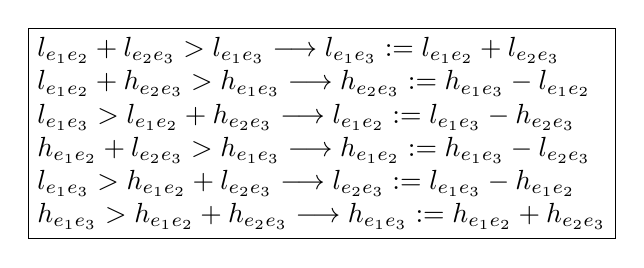
\begin{tikzpicture}[every text node part/.style={align=left}]
        \node (n1) at (0,0) [rectangle, draw]
        {
%        \begin{gather*}
 $\Low{e_1}{e_2} + \Low{e_2}{e_3} > \Low{e_1}{e_3}
  \longrightarrow \Low{e_1}{e_3} := \Low{e_1}{e_2} + \Low{e_2}{e_3}$\\

   $\Low{e_1}{e_2} + \High{e_2}{e_3} > \High{e_1}{e_3}
 \longrightarrow \High{e_2}{e_3} := \High{e_1}{e_3} - \Low{e_1}{e_2}$\\

  $\Low{e_1}{e_3} > \Low{e_1}{e_2} + \High{e_2}{e_3}
  \longrightarrow \Low{e_1}{e_2} := \Low{e_1}{e_3} - \High{e_2}{e_3}$\\

 $\High{e_1}{e_2} + \Low{e_2}{e_3} > \High{e_1}{e_3}
 \longrightarrow \High{e_1}{e_2} := \High{e_1}{e_3} - \Low{e_2}{e_3}$\\

$\Low{e_1}{e_3} > \High{e_1}{e_2} + \Low{e_2}{e_3}
  \longrightarrow \Low{e_2}{e_3} := \Low{e_1}{e_3} - \High{e_1}{e_2}$\\

 $\High{e_1}{e_3} > \High{e_1}{e_2} + \High{e_2}{e_3}
 \longrightarrow \High{e_1}{e_3} := \High{e_1}{e_2} + \High{e_2}{e_3}$
%\end{gather*}
               };
            %  \node (n1) at (0,-1.1) [rectangle, draw = none]{$\gamma$};
      \end{tikzpicture}
      %  \end{center}
 %       };
      \caption{Rules for stabilising a distance relation}
\label{fig-rules}
\vspace{-5mm}
    \end{minipage}}
\adjustbox{valign=b}
 {\begin{minipage}{0.37\linewidth}
\adjustbox{valign=b}
 {\begin{minipage}{0.49\linewidth}
 \begin{center}
 %               \adjustbox{valign=b}
%{\begin{minipage}{0.49\linewidth}
  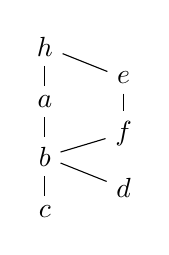
\begin{tikzpicture}
    \tikzset{vertex/.style = {shape=circle,draw,minimum size=1em}}
    \tikzset{vertex3/.style = {shape=circle,draw,minimum size=1.5em}}
    \tikzset{vertex2/.style = {shape=rectangle,draw=none,minimum size=0.5em}}
    \tikzset{edge/.style = {-,> = latex'}}

    % vertices

    \node[vertex2] (b) at  (0,-0.7) {$h$};

    \node[vertex2] (x) at  (0,-1.4) {$a$};
\node[vertex2] (y) at  (1,-1.1) {$e$};
\node[vertex2] (z) at  (1,-1.8) {$f$};
    \node[vertex2] (e) at  (0,-2.1) {$b$};

    \node[vertex2] (f) at  (0,-2.8) {$c$};
   \node[vertex2] (g) at  (1,-2.5) {$d$};
       %edges
  %  \draw[edge] (b) to node[right ]{$[0]$} node[left]{$a$} (x);
 \draw[edge] (b) to (x);
    \draw[edge] (x) to (e);
    \draw[edge] (e) to (f);
   %  \draw[edge] (e) to (g);
      \draw[edge] (b) to (y);
       \draw[edge] (y) to (z);
        \draw[edge] (z) to (e);
        \draw[edge] (e) to (g);
    \end{tikzpicture}
 %    \caption{$\PR{\DScenario}$}
   %  maximal chains ($\DScenario_1$)}
%     \label{fig-chains}
     \end{center}
    \end{minipage}}
    \adjustbox{valign=b}
     {\begin{minipage}{0.49\linewidth}
 \begin{center}
 %               \adjustbox{valign=b}
%{\begin{minipage}{0.49\linewidth}
  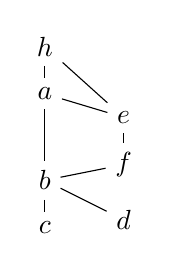
\begin{tikzpicture}
    \tikzset{vertex/.style = {shape=circle,draw,minimum size=1em}}
    \tikzset{vertex3/.style = {shape=circle,draw,minimum size=1.5em}}
    \tikzset{vertex2/.style = {shape=rectangle,draw=none,minimum size=0.5em}}
    \tikzset{edge/.style = {-,> = latex'}}

    % vertices

    \node[vertex2] (b) at  (0,-0.3) {$h$};

    \node[vertex2] (x) at  (0,-0.9) {$a$};
\node[vertex2] (y) at  (1,-1.2) {$e$};
\node[vertex2] (z) at  (1,-1.8) {$f$};
    \node[vertex2] (e) at  (0,-2) {$b$};
    \node[vertex2] (f) at  (0,-2.6) {$c$};
   \node[vertex2] (g) at  (1,-2.5) {$d$};
       %edges
  %  \draw[edge] (b) to node[right ]{$[0]$} node[left]{$a$} (x);
 \draw[edge] (b) to (x);
    \draw[edge] (x) to (e);
    \draw[edge] (e) to (f);
     \draw[edge] (x) to (y);
      \draw[edge] (b) to (y);
       \draw[edge] (y) to (z);
        \draw[edge] (z) to (e);
        \draw[edge] (e) to (g);
    \end{tikzpicture}
 %    \caption{$\PR{\DScenario}$}
   %  maximal chains ($\DScenario_1$)}
 %    \label{fig-chains}
     \end{center}
    \end{minipage}}
 \caption{$\PR{\DScenario_1}$ and $\ParSE{\DScenario_1}$}
   %  maximal chains ($\DScenario_1$)}
     \label{fig-chains}
     \vspace{-5mm}
 \end{minipage}}
   \end{center}
  \end{figure}
%-----------------------


We represent a partial order by its maximal chains, visually
represented by a Hasse diagram. For $\DScenario_1$,
$\PR{\DScenario_1}$ is shown in \Fig{fig-chains},
%The stable distance function of $\DScenario_1$,
$\DFS{\DScenario_1}$ is represented by
$\{(h, a, 0, 3),
(h, b, 4, 7),
(h, c, 4, \infty),
(h, d, 4, \infty),
(h, e, 4, 7),
(h, f, 4, 7),
(a, b, 1, 4),\\
(a, c, 1, \infty),
(a, d, 1, \infty),
(e, b, 0, 3),
(e, f, 0, 3),
(f, b, 0, 3)\}$.
Tuples of the form\\ $(e,e',0,\infty)$ (indicating default
constraints) will not be included in our examples.
%----------------------------

{\bf Extended distance relations}
The \emph{extended partial order} of $\DScenario$,
$\ParSE{\DScenario}: \Sigma_{\DScenario} \times  \Sigma_{\DScenario}$,
is the smallest relation
that satisfies the following conditions: (i) if
$e\PR{\DScenario}e'$, then $e\ParSE{\DScenario}e'$; (ii) if there
exists $o\in\Sigma_{\DScenario}$ such that $o\ParSE{\DScenario}e$,
$o\ParSE{\DScenario}e'$ and $\Max{o}{e} < \Min{o}{e'}$
 in $\DFS{\DScenario}$,
or $e\ParSE{\DScenario}o$, $e'\ParSE{\DScenario}o$ and $\Max{e'}{o}
< \Min{e}{o}$ in $\DFS{\DScenario}$, then $e\ParSE{\DScenario}e'$;
(iii) if $e\ParSE{\DScenario}e'$ and  $e'\ParSE{\DScenario}e''$, then
$e\ParSE{\DScenario}e''$.
%the transitive closure of $\ParS{\DScenario}$
The \emph{initial} extended distance relation of \DScenario{} is
%  $\DRS{\DScenario}=(\PR{\DScenario},\DFS{\DScenario})$ is
 $\DRE{\DScenario}=(\ParSE{\DScenario},\DFEX{\DScenario})$,
where
    $\DFEX{\DScenario}(e, e') = [0,\infty]$ if
$(e,e')$ in $\ParSE{\DScenario}\setminus \ParS{\DScenario}$,
and $\DFEX{\DScenario}(e, e') = \DFS{\DScenario}(e, e')$ if
 $(e,e')$ in $\ParS{\DScenario}$.
The \emph{stable extended distance relation} of $\DScenario$,
denoted by $\DRSE{\DScenario}=(\ParSE{\DScenario},\DFE{\DScenario})$, is
obtained by stabilising $\DRE{\DScenario}$.

In $\DScenario_1$, $\Max{h}{a}=3 < \Min{h}{e}=4$ in $\DFS{\DScenario_1}$,
so $\PR{\DScenario_1}$ can be extended with $(a,e)$ (see
$\ParSE{\DScenario_1}$ in \Fig{fig-chains}) and
$\DFE{\DScenario_1}=\DFS{\DScenario_1}\cup\{(a,e,1,4),(a,f,1,4)\}$.

To avoid visual clutter
%in the rest of the text,
we will use
$\DR{\DScenario}=(\ParS{\DScenario},\DF{\DScenario})$ for the stable
extended distance relation of $\DScenario$.
A (sequential) scenario, $\xi$, can be seen as a trivial DTS,
$\D(\xi)$. We use $\DR{\xi}=(\ParS{\xi},\DF{\xi})$ for its stable
distance relation, where $\PR{\xi}$ is $\TotalS{\xi}$.

%\noindent
{\bf Realisability of (sequential) scenarios as distributed
scenarios}
Let $\mathcal{S}=\{\SeqS_1,\dots,\SeqS_n\}$, such that each
$\SeqS_i\in\mathcal{S}$ has a
different sequence of events, and
each event in $\Sigma_{\mathcal{S}}$ occurs exactly once in each $\SeqS_i$.
If there exists a DTS
$\DScenario$ over $\Sigma_{\mathcal{S}}$, such
that $\Sem{\DScenario} = \bigcup_{1\leq i \leq
n} \Sem{\SeqS_{i}}$, we say $\mathcal{S}$ is \emph{realisable} by
$\DScenario$.

%----------------------
{\bf Projections of distance relations}
Let $\DR{}=(\ParS{},\DF{})$ be a
stable distance relation over $\Sigma$.
A \emph{projection} of $\DR{}$ is a
scenario $\xi_p = (p, \C_p)$, where
(i) $p$ is a permutation of events in $\Sigma$ that
agrees with $\ParS{}$, and
(ii) $\C_{p}$ is a set of constraints:
for every $e$ and $e'$ such that $e$ appears before
$e'$ in $p$,
if $e\not\ParS{}e'$, then the default constraints
$0 \leq \TT{e}{e'}\leq \infty$ are added to $\C_p$,
otherwise the constraints
$l \leq \TT{e}{e'} \leq h$ are added to $\C_{p}$, where
$\DF{}(e,e')=[l,h]$.
When we create $\DR{\xi_p}$, we must, of course, stabilise it.
In the rest of the text we assume the distance relations of all
the projections are stabilised.

The set of all the projections obtained in this way is realisable by
any DTS for which $\DR{}$ is the extended distance relation.
Moreover, given the extended distance relation $\DR{}$ for a DTS
\DScenario, the set of projections of $\DR{}$ uniquely determines the
semantics of \DScenario: every behaviour in $\Sem{\DScenario}$ is allowed by
one projection.
%-------------------------------

%----------------------------------
%\vspace{-2em}
\section{Timed Scenario Expressions}
\label{sec-exp}
%\input{expressions}
In this section we introduce the notion of timed scenario expressions
(expressions for short). Expressions allow us to construct models of
behaviours of complicated systems whose constituent parts are
distributed
systems. They provide a hierarchical way of specifying systems, where
distributed scenarios are used as the building blocks.
First, we introduce a few operations for manipulating scenarios.
%\vspace{-0.5em}
\begin{definition}
  \label{def-comp-par-seq}
Let $\xi=(\E_1,\C_1)$ and $\eta=(\E_2,\C_2)$ be two normalised scenarios
over $\Sigma_\xi$ and $\Sigma_\eta$, respectively.
 \setlist{nolistsep}
\begin{itemize}[noitemsep]
%\begin{itemize}
  \item
The \emph{concatenation} of
$\xi$ and $\eta$, denoted by $\xi\circ\eta$, is
defined if $\Sigma_\xi\cap\Sigma_\eta=\emptyset$.
If defined, $\xi\circ\eta$ is the scenario
$(\E,\C_1\cup\C_2)$ over $\Sigma_\xi\cup\Sigma_\eta$, where $\E$ is
the concatenation of $\E_1$ and $\E_2$.
The semantics of $\xi\circ\eta$, denoted by $\Sem{\xi\circ\eta}$, is
$\Sem{\xi}\circ\Sem{\eta}$, that is, every behaviour of $\xi \circ \eta$
is a concatenation of some behaviour of $\xi$ and some behaviour of
$\eta$.
\item
   The \emph{choice} between two alternatives, $\xi$ and $\eta$, is denoted by
   $\xi\BAR\eta$.
   Its semantics is defined by $\Sem{\xi\BAR\eta} = \Sem{\xi}\cup\Sem{\eta}$.
\end{itemize}
\end{definition}
\noindent
If $\xi$ and $\eta$ are two scenarios, then
$\xi\BAR\eta$ is consistent if $\xi$ or $\eta$ is consistent.
If $\xi\circ\eta$ is defined, then it is consistent
%, i.e., $\Sem{\xi\circ\eta}\neq \emptyset$
if $\xi$ and $\eta$ are both consistent.

%, and $\xi||\eta$ is consistent if the DTS $\DScenario=\{\xi,\eta\}$
%is consistent.

%It is worth mentioning that the semantics of the operator $||$ is
%in accordance with the rendezvous synchronisation semantics of a DTS
%(see \Sec{sec-dts}): the semantics of a DTS is obtained by the
%parallel composition of its components.
%----------------
%\begin{obs}
%   \label{obs-comp-par-seq}
%Let $\xi$ and $\eta$ be two consistent scenarios. Then,

%$\Sem{\xi\circ\eta} = \Sem{\xi}\circ\Sem{\eta}$ and
%%$\Sem{\xi||\eta} =
%%\Sem{\DScenario}$, where $\DScenario=\{\xi,\eta\}$ is a DTS, and
%$\Sem{\xi\BAR\eta} =
%\Sem{\xi}\cup\Sem{\eta}$.
%\end{obs}
%----------------
%\vspace{-0.5em}
\begin{definition}
   \label{def-comp-par-alt-dts}
Let $\DScenario_1=\D(\xi_1,\dots,\xi_n)$ and
$\DScenario_2=\D(\eta_1,\dots,\eta_m)$ be two distributed
scenarios over $\Sigma_{\DScenario_1}$ and $\Sigma_{\DScenario_2}$,
respectively.
 \setlist{nolistsep}
\begin{itemize}[noitemsep]
%\begin{itemize}
  \item
The \emph{concatenation} of
$\DScenario_1$ and $\DScenario_2$, denoted by
$\DScenario_1\circ\DScenario_2$, is defined if
$\Sigma_{\DScenario_1}\cap\Sigma_{\DScenario_2}=\emptyset$.
If defined, $\DScenario_1\circ\DScenario_2$ is
the DTS
$\DScenario=\D(\gamma_{11},\dots,\gamma_{1m},\dots,\gamma_{n1},\dots,\gamma_{nm})$
over
$\Sigma_{\DScenario_1}\cup\Sigma_{\DScenario_2}$, where
$\gamma_{ij}=\xi_i\circ\eta_j$ (for $1\leq i\leq n$
and $1\leq j\leq m$),
and
%The semantics of $\DScenario_1\circ\DScenario_2$, denoted by
$\Sem{\DScenario_1\circ\DScenario_2}=\Sem{\DScenario}$.
%, is $\Sem{\DScenario_1}\circ\Sem{\DScenario_2}$.
\item
  The \emph{parallel composition} of $\DScenario_1$, and
  $\DScenario_2$, denoted by $\DScenario_1||\DScenario_2$, is the DTS
  $\DScenario=\D(\xi_1,\dots,\xi_n,\eta_1,\dots,\eta_m)$
  over $\Sigma_{\DScenario_1}\cup\Sigma_{\DScenario_2}$ and
  $\Sem{\DScenario_1||\DScenario_2} =\Sem{\DScenario}$.
\item
   The \emph{choice} between two alternatives,
$\DScenario_1$ and $\DScenario_2$, is denoted by
$\DScenario_1\BAR\DScenario_2$.
Its semantics is defined by $\Sem{\DScenario_1\BAR\DScenario_2} =
 \Sem{\DScenario_1}\cup\Sem{\DScenario_2}$.
  \end{itemize}
\end{definition}
%---------------
\noindent
If $\DScenario_1$ and $\DScenario_2$ are two distributed scenarios,
then $\DScenario_1\BAR\DScenario_2$ is consistent if $\DScenario_1$ or
$\DScenario_2$ is consistent.
If $\DScenario_1\circ\DScenario_2$ is defined, then it is consistent
if $\DScenario_1$ and $\DScenario_2$ are both consistent.
It is worth pointing out that, except for the case of concatenation,
$\DScenario_1$ and $\DScenario_2$ might share some event names. In
that case, the event names in
$\Sigma_{\DScenario_1}\cap\Sigma_{\DScenario_2}$ will be synchronising
events in $\DScenario_1||\DScenario_2$. If $\DScenario_1$ and
$\DScenario_2$ are both consistent, $\DScenario_1||\DScenario_2$
might not be well-formed, and, if well-formed, might not be consistent.

For example, $\DScenario_1 = \D(\xi_1,\xi_2)$, where
 $\xi_1 = (abc, \{\TT{a}{b} \geq 2\})$ and $\xi_2 =
 (eb, \{\TT{e}{b} \leq 3\})$ is a consistent DTS, so is
$\DScenario_2 = \D(\xi_3)$, where
 $\xi_3 = (efb, \{\TT{e}{b} \geq 4\})$. But
$\DScenario_1||\DScenario_2$ is inconsistent. Observe that $b$ is a
synchronising event in $\DScenario_1$, while both $b$ and $e$ are the
synchronising events in $\DScenario_1||\DScenario_1$. Because the
constraints $\TT{e}{b} \leq 3$ in $\DScenario_1$ and $\TT{e}{b}
\geq 4$ in $\DScenario_2$ cannot be satisfied simultaneously,
$\DScenario_1||\DScenario_1$ is inconsistent.
%----------------
%\begin{obs}
%   \label{obs-comp-par}
%Let $\DScenario_1$ and $\DScenario_2$ be two consistent distributed
%scenarios. Then,
%$\Sem{\DScenario_1\circ\DScenario_2} =
%\Sem{\DScenario_1}\circ\Sem{\DScenario_2}$,
%$\Sem{\DScenario_1||\DScenario_2} =
%\Sem{\DScenario}$, where
%$\DScenario=\D(\xi_1,\dots,\xi_n,\eta_1,\dots,\eta_m)$ is a DTS,
%$\DScenario_1=\D(\xi_1,\dots,\xi_n)$ and
%$\DScenario_2=\D(\eta_1,\dots,\eta_m)$,
%and
%$\Sem{\DScenario_1\BAR\DScenario_2} =
%\Sem{\DScenario_1}\cup\Sem{\DScenario_2}$.
%\end{obs}
%--------------
%\vspace{-0.5em}
\begin{definition}
  \label{def-simple-exp}
 % $S$ is a \emph{timed scenario expression} (\emph{expression}
 % for short), if $S$ is
  A \emph{timed scenario expression} (\emph{expression}
  for short) is one of the following:
  \setlist{nolistsep}
\begin{itemize}[noitemsep]
  \item
    a DTS,
    %xsequential scenario,
  \item
    $(E_1\circ E_2)$, where $E_1$ and $E_2$ are
    expressions,
  \item
    $(E_1||E_2)$, where $E_1$ and $E_2$ are
    expressions, or
    \item
      $(E_1\BAR E_2)$, where $E_1$ and $E_2$ are  expressions.
 %     \item
 %   $E_1^*$, where $E_1$ is a scenario expression.
  \end{itemize}
  \end{definition}
%------------------
\noindent
Recall that a scenario $\xi$ can be seen as the DTS
$\D(\xi)$, so it is an expression.
%In our expressions we are going to treat a sequential
%scenario as a DTS with one component.

It should be obvious that the three operators, $\circ$, $\BAR$ and $||$,
are associative. The first one is not commutative, while the other two
are.

The following observation follows directly from the definitions.
%-----------------
%\vspace{-0.5em}
\begin{obs}
  \label{obs-dist-laws}
  Distributive laws for  expressions:
   \setlist{nolistsep}
\begin{itemize}[noitemsep]
%  \begin{itemize}
  \item
    $E_1\circ(E_2||E_3)=(E_1\circ E_2)||(E_1\circ E_3)$,
  %  \item
      $(E_1||E_2)\circ E_3=(E_1\circ E_3)||(E_2\circ E_3)$
       \item
         $E_1\circ(E_2\BAR E_3)=(E_1\circ E_2)\BAR(E_1\circ E_3)$,
    %     \item
           $(E_1\BAR E_2)\circ E_3=(E_1\circ E_3)\BAR(E_2\circ E_3)$
            \item
              $E_1||(E_2\BAR E_3)=(E_1||E_2)\BAR(E_1||E_3)$,
           %    \item
      $(E_1\BAR E_2)||E_3=(E_1||E_3)\BAR(E_2||E_3)$
    \end{itemize}
  \end{obs}
%-------------------------
%\vspace{-0.5em}
\begin{definition}
  \label{def-simple-normal-form}
  An expression, $E$, is in \emph{normal form} if $E$ is
  either a DTS $\DScenario$, or of the form
  $\DScenario_1\BAR\dots\BAR\DScenario_k$, where each $\DScenario_i$
  ($1\leq i\leq k, 1<k$) is a DTS.
\end{definition}
\noindent
Using the distributive laws an
expression can be converted into normal form. It should be obvious
that the normal form of an expression is unique.
%---------------
%\vspace{-0.5em}
\begin{obs}
  \label{obs-exp-sem}
Let $E$ be an expression. The semantics of $E$, denoted by
$\Sem{E}$, is
 \setlist{nolistsep}
\begin{itemize}[noitemsep]
%\begin{itemize}
  \item
  $\Sem{\DScenario}$, if $E$ is an
  expression with normal form $\DScenario$,
\item
  $\Sem{\DScenario_1}\cup\dots\cup\Sem{\DScenario_k}$, if $E$ is an
   expression with normal form $\DScenario_1\BAR\dots\BAR\DScenario_k$
  ($1<k$).
%\item
%  $\Sem{E_1}\cup\Sem{E_2}$, if $S$ is of the form $(E_1\BAR E_2)$, where
%  $E_1$ and $E_2$ are expressions.
\end{itemize}
\end{obs}
%---------------
%\noindent
%--------------
%\vspace{-0.5em}
\begin{definition}
  \label{def-valid}
An expression, $E$, is \emph{consistent}, if
$\Sem{E}\neq\emptyset$.
  \end{definition}
\noindent
If $E$ is a consistent expression,
we say $\Sem{E}$ is the set of behaviours that are \emph{described} or
\emph{expressed} by $E$.
%-------------------
%\vspace{-0.5em}
\begin{example}
\label{ex-race}
Consider a system in which two runners compete with each other
in a race managed by a controller \cite{Beek-2023}. The race begins with the
controller issuing a signal {\tt start}, which is received by both the
runners simultaneously.
Upon completing the run, runner $\mathtt{i}$ sends a $\mathtt{finish_i}$ signal
to the controller.
So there are two alternative outcomes, depending on
which runner finishes first.
This can be modeled by the expression $\mathtt{(C_1\BAR C_2)||R_1||R_2}$,
in which $\mathtt{C_1}$ and $\mathtt{C_2}$ correspond to the two
%alternative
outcomes, each specified by a DTS:
$\mathtt{C_1}=(\mathtt{start}~ \mathtt{finish_1}~ \mathtt{finish_2},\emptyset)$,
$\mathtt{C_2}=(\mathtt{start}~ \mathtt{finish_2}~ \mathtt{finish_1},\emptyset)$,
while $\mathtt{R_1}$ and $\mathtt{R_2}$ capture
the behaviours of the runners:
$\mathtt{R_1}=(\mathtt{start}~ \mathtt{finish_1},\emptyset)$,
$\mathtt{R_2}=(\mathtt{start}~ \mathtt{finish_2},\emptyset)$.
%as shown in \Fig{fig-race}.
Observe that %because events are instantaneous,
{\tt start} is
a synchronising event between all the components,
$\mathtt{finish_1}$ is a synchronising event between the controller
(specified by $\mathtt{(C_1\BAR C_2)}$) and $\mathtt{R_1}$,
while $\mathtt{finish_2}$ is a synchronising event between the controller
and $\mathtt{R_2}$.
  \end{example}
\noindent
In the rest of the paper our examples will not feature the operator $\circ$, as
it plays no role in the problem of realisation.

%----------------------------------
%\vspace{-1em}
\section{Realisation of Sequential Scenarios as Expressions}
\label{sec-realize}
In our earlier work \cite{DTS-2025} we addressed the question of whether
a set $\mathcal{S}$ of normalised (sequential) scenarios, whose
sequences of events are different permutations of the same set, can be
realised as a single DTS that is
semantically equivalent to $\mathcal{S}$, i.e., describes the same set of
behaviours as $S$. This can be done only if there is a distance
relation whose set of projections is the same as $\mathcal{S}$. We
showed how to obtain such a distance relation and a corresponding
DTS \cite{DTS-2025}.
%(see \Sec{sec-dts} for a brief summary).

In this section we tackle the problem of realisability of
scenarios \emph{as expressions}: given a set, $\mathcal{S}$,
of scenarios, we want to find an expression that realises
$\mathcal{S}$.
Despite similarities, there is a fundamental difference between
this problem and the one previously solved \cite{DTS-2025}: the
members of $\mathcal{S}$ could be projections that are obtained from
extended distance relations of different distributed
scenarios, in which case $\mathcal{S}$ cannot be realised by a single
DTS, but by a choice expression that involves more than one DTS. The
challenge is to divide $\mathcal{S}$ in such a way that each
partition could be realised by a DTS, while trying to avoid the trivial
solution in which every member of S is a separate alternative.
More precisely:
\vspace{-0.5em}
\begin{quote}
Given a finite set $\mathcal{S}=\{\SeqS_1,\dots,\SeqS_n\}$ of
scenarios of \emph{possibly different lengths} over
$\Sigma$, such that
(i) $\ESeq{\SeqS_i}\neq \ESeq{\SeqS_j}$ (for $1\leq
i,j\leq n$ and $i\neq j$)\footnote{In \Sec{sec-relax} we
show how to relax the assumption.}, and (ii)
each event of $\SeqS_i$ ($1\leq i\leq n$) has a
unique occurrence in $\SeqS_i$,
we want to obtain an expression $E$
over $\Sigma$, such that $\Sem{E} = \Sem{\mathcal{S}}=\bigcup_{1\leq
i \leq n} \Sem{\SeqS_i}$.
In general, $\mathcal{S}$ can be realised by more than one
expression.
Our goal is to find an expression with a
reasonably small number of alternatives, while decreasing the number
of trivial alternatives.
\end{quote}
\vspace{-0.6em}
We say $\mathcal{S}$ is \emph{realisable by} $E$, or
$E$ is a \emph{realisation} of $\mathcal{S}$, if $\mathcal{S}$ is
realised by $E$.
\vspace{-0.2em}
\begin{example}
\label{ex-one-flag}
Given the set, $\mathcal{S}=\{\SeqS_1,\SeqS_2,\SeqS_3,\SeqS_4\}$, of
scenarios, where

\noindent
$\SeqS_1=(\mathtt{start}~ \mathtt{finish_1}~ \mathtt{finish_2}~ \mathtt{flag_1},\emptyset)$,
$\SeqS_2=(\mathtt{start}~ \mathtt{finish_1}~  \mathtt{flag_1}~ \mathtt{finish_2},\emptyset)$,
$\SeqS_3=(\mathtt{start}~ \mathtt{finish_2}~ \mathtt{finish_1}~ \mathtt{flag_2},\emptyset)$,
%and
$\SeqS_4=(\mathtt{start}~ \mathtt{finish_2}~ \mathtt{flag_2}~ \mathtt{finish_1},\emptyset)$,
there is no DTS that realises $\mathcal{S}$.
But $\mathcal{S}$ can be divided into two sets
$\mathcal{S}_{1}=\{\SeqS_1,\SeqS_2\}$ and
$\mathcal{S}_2=\{\SeqS_3,\SeqS_4\}$ based on the sets of events of its
members. The set ${\mathcal{S}}_{1}$ can be realised by DTS
$E=\D(\xi_1,\xi_2)=\xi_1||\xi_2$, where
$\xi_1=(\mathtt{start}~ \mathtt{finish_1}~ \mathtt{flag_1},\emptyset)$
and
$\xi_2=(\mathtt{start}~ \mathtt{finish_1}~ \mathtt{finish_2},\emptyset)$.
Similarly, $\mathcal{S}_2$ is realised by DTS
$E'=\xi_3||\xi_4$, where
$\xi_3=(\mathtt{start}~ \mathtt{finish_2}~ \mathtt{flag_2},\emptyset)$
and
$\xi_4=(\mathtt{start}~ \mathtt{finish_2}~ \mathtt{finish_1},\emptyset)$.
So $\mathcal{S}$ is realised by the expression
$E\BAR E'=(\xi_1||\xi_2)|(\xi_3||\xi_4)$.
\end{example}
\vspace{-0.5em}
%------------------------
\begin{definition}
  \label{def-DR-S}
Let $\mathcal{S}=\{\SeqS_1,\dots,\SeqS_n\}$ be a finite set of
normalised scenarios
%over $\Sigma_{\mathcal{S}}$
and
$\{\DR{\SeqS_1},\dots,\DR{\SeqS_n}\}$ be the set of
corresponding stable distance relations, where
$\DR{\SeqS_i}=(\PR{\SeqS_i},\DF{\SeqS_i})$ ($1\leq i\leq n$).
\emph{The distance relation of} $\mathcal{S}$, $\DR{\mathcal{S}}$, is
the pair $(\ParS{\mathcal{S}},\DF{\mathcal{S}})$, where
$\ParS{\mathcal{S}}=\bigcap_{1\leq i\leq n} \PR{\SeqS_i}$ and,
for every $(e,e')$ in $\ParS{\mathcal{S}}$,
$\DF{\mathcal{S}}(e,e')$ is
the smallest interval that includes each $\DF{\SeqS_i}(e,e')$.
%$\DR{\mathcal{S}}$ is stable and cannot be extended.
\end{definition}
\vspace{-0.3em}
\noindent
The first step\label{initial-partitioning-step}
 in solving the problem posed at the beginning of this
section is to divide
$\mathcal{S}$ in such a way that all the members of each partition are
scenarios of equal lengths over the same set of events.
Then we solve the problem for each partition, independently.
Our general strategy is the following: whenever a partition is not
realisable by a single DTS, we divide it
%If a partition is not realisable by a single DTS, we divide it
repeatedly, so that at the end each partition will be realised by a
DTS and will correspond to one alternative in the overall choice expression.
This process is guided by the results of our analysis based on
$\PR{\mathcal{S}}$ and
%the constraints of $\mathcal{S}$,
$\DF{\mathcal{S}}$,
described in sections \ref{sec-no-time}
and \ref{sec-full}. Additionally, some divisions are simply necessary, as
described below.
%But first, an important definition:
%-------------
\vspace{-1em}
\subsubsection{Gaps}\label{paragraph-gaps}
Let $S_{(e, e')}=\{s_i\in \mathcal{S}|e\PR{\SeqS_i}e'\}$.
Let $s_1,\dots,s_m$ be a sequence of members of $S_{(e, e')}$ such
that, for every $1\leq i\leq m$, $[l_i, h_i]=\DF{s_i}(e, e’)$
and $l_i \leq l_{i+1}$.
Let $H_{r}=\max \{h_j|1\leq j \leq r\}$.
If there is a $k$, $1 \leq k < m$, such that
$H_{k} < l_{k+1}$, $\DF{S}(e, e’)$ contains a gap.
Then $\mathcal{S}$ is said to be \emph{with gaps}.
An $\mathcal{S}$ with gaps cannot be realised by a single DTS:
this is because the interval between $e$ and $e'$ in
$\DF{\mathcal{S}}$ would be
$[l_1,H_{m}]$, which would allow also behaviours
 in which the time distance
 between $e$ and $e'$ is between $H_k$ and $l_{k+1}$. Such behavious are
  allowed by none of the members of $\mathcal{S}$.
  So $\mathcal{S}$ must be divided into partitions with no gaps.
%, but would be allowed by any expression that realises $\mathcal{S}$.

Whenever a partition is divided into finer partitions (see \Sec{sec-no-time}
 and \Sec{sec-full}), we must check for the existence of gaps in any
 newly formed partition.%  (see \Sec{sec-algo}).% and divide accordingly.


% In general, it might be necessary to divide a partition further into
% subgroups (see \Sec{sec-no-time}
% and \Sec{sec-full}). So we must check for the existence of gaps in
% any newly formed partition and divide accordingly.

In the rest of the paper we assume that all scenarios in
$\mathcal{S}$ are over the same set, $\Sigma_{\mathcal{S}}$, of
events, and that each $\SeqS\in\mathcal{S}$
contains all the events from $\Sigma_{\mathcal{S}}$.
Moreover, we assume that any divisions necessitated by
gaps have already been carried out, so that $\mathcal{S}$ is without gaps.
%, and moreover the intervals of $\DF{\mathcal{S}}$ are without gaps.
We describe our method in two steps:
%in the first step
first, we tackle the
problem \emph{without accounting for constraints}.
Because constraints will not play a role,
in our examples we will discuss scenarios with only default constraints.
%we assume each member of $\mathcal{S}$ is of the form
%$(\E,\emptyset)$: it has only default constraints.
%---------------

%---------------------------------
%\vspace{-0.5em}
\subsection{Partitioning a Set of Sequential Scenarios Based on
Ordering}
\label{sec-no-time}
Let $\mathcal{S}=\{\SeqS_1,\dots\SeqS_n\}$ be a set of normalised
scenarios over $\Sigma_{\mathcal{S}}$, such that, for every $1\leq
i\leq n$, $\SeqS_i=(\E_i,\emptyset)$, where $\E_i$
%over $\Sigma_{\mathcal{S}}$, whose members
contains all the events from $\Sigma_{\mathcal{S}}$. Moreover, let
$\mathcal{S}$ be without gaps. We are interested
in obtaining an expression that realises $\mathcal{S}$.
%First, we show a simple example.
%---------------
\begin{figure}[t]
\begin{center}
\adjustbox{valign=b}
 {\begin{minipage}{0.41\linewidth}
 \begin{center}
 %               \adjustbox{valign=b}
%{\begin{minipage}{0.49\linewidth}
  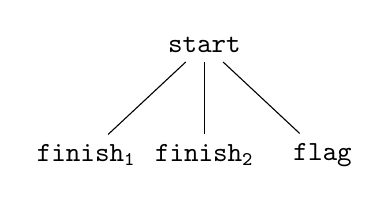
\begin{tikzpicture}
    \tikzset{vertex/.style = {shape=circle,draw,minimum size=1em}}
    \tikzset{vertex3/.style = {shape=circle,draw,minimum size=1.5em}}
    \tikzset{vertex2/.style = {shape=rectangle,draw=none,minimum size=0.5em}}
    \tikzset{edge/.style = {-,> = latex'}}

    % vertices

    \node[vertex2] (b) at  (0,0) {$\mathtt{start}$};

    \node[vertex2] (x) at  (-1.5,-1.4) {$\mathtt{finish_1}$};
\node[vertex2] (y) at  (0,-1.4) {$\mathtt{finish_2}$};
\node[vertex2] (z) at  (1.5,-1.4) {$\mathtt{flag}$};
 \draw[edge] (b) to (x);
    \draw[edge] (b) to (y);
    \draw[edge] (b) to (z);
      \end{tikzpicture}
     \caption{Maximal chains (Example \ref{ex-one-same-flag})}
     \label{fig-chains-1}
      \vspace{-3mm}
     \end{center}
    \end{minipage}}
    \adjustbox{valign=b}
        {\begin{minipage}{0.58\linewidth}
         \begin{center}
 %               \adjustbox{valign=b}
%{\begin{minipage}{0.49\linewidth}
 \adjustbox{valign=b}
        {\begin{minipage}{0.49\linewidth}
  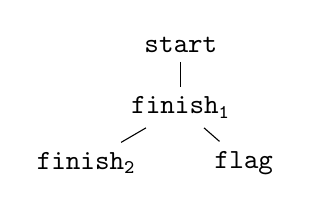
\begin{tikzpicture}
    \tikzset{vertex/.style = {shape=circle,draw,minimum size=1em}}
    \tikzset{vertex3/.style = {shape=circle,draw,minimum size=1.5em}}
    \tikzset{vertex2/.style = {shape=rectangle,draw=none,minimum size=0.5em}}
    \tikzset{edge/.style = {-,> = latex'}}

    % vertices

    \node[vertex2] (b) at  (0.2,-0.2) {$\mathtt{start}$};

    \node[vertex2] (x) at  (0.2,-1) {$\mathtt{finish_1}$};
\node[vertex2] (y) at  (-1,-1.7) {$\mathtt{finish_2}$};
\node[vertex2] (z) at  (1,-1.7) {$\mathtt{flag}$};
 \draw[edge] (b) to (x);
 %   \draw[edge] (b) to (y);
    \draw[edge] (x) to (z);
     \draw[edge] (x) to (y);
      \end{tikzpicture}
       \end{minipage}}
        \adjustbox{valign=b}
        {\begin{minipage}{0.49\linewidth}
  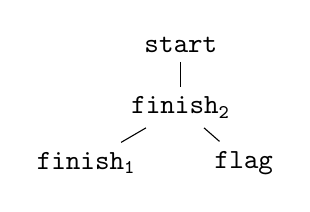
\begin{tikzpicture}
    \tikzset{vertex/.style = {shape=circle,draw,minimum size=1em}}
    \tikzset{vertex3/.style = {shape=circle,draw,minimum size=1.5em}}
    \tikzset{vertex2/.style = {shape=rectangle,draw=none,minimum size=0.5em}}
    \tikzset{edge/.style = {-,> = latex'}}

    % vertices

    \node[vertex2] (b) at  (0.2,-0.2) {$\mathtt{start}$};

    \node[vertex2] (x) at  (0.2,-1) {$\mathtt{finish_2}$};
\node[vertex2] (y) at  (-1,-1.7) {$\mathtt{finish_1}$};
\node[vertex2] (z) at  (1,-1.7) {$\mathtt{flag}$};
 \draw[edge] (b) to (x);
  %  \draw[edge] (b) to (y);
    \draw[edge] (x) to (z);
     \draw[edge] (x) to (y);
      \end{tikzpicture}
       \end{minipage}}
     \caption{Maximal chains for $\ParS{\mathcal{S}_1}$,
    $\ParS{\mathcal{S}_2}$(Example \ref{ex-one-same-flag})}
     \label{fig-chains-2}
     \vspace{-3mm}
     \end{center}
    \end{minipage}}
  \end{center}
  \end{figure}
%-----------------------
\vspace{-1em}
\begin{example}
\label{ex-one-same-flag}
%Consider the set $\mathcal{S}=\{\SeqS_1,\SeqS_2,\SeqS_3,\SeqS_4\}$, of
%scenarios, where
Let $\mathcal{S}=\{\SeqS_1,\SeqS_2,\SeqS_3,\SeqS_4\}$, where
%\noindent
$\SeqS_1=(\mathtt{start}~ \mathtt{finish_1}~ \mathtt{finish_2}~ \mathtt{flag},\emptyset)$,
$\SeqS_2=(\mathtt{start}~ \mathtt{finish_1}~  \mathtt{flag}~ \mathtt{finish_2},\emptyset)$,
$\SeqS_3=(\mathtt{start}~ \mathtt{finish_2}~ \mathtt{finish_1}~ \mathtt{flag},\emptyset)$
and
$\SeqS_4=(\mathtt{start}~ \mathtt{finish_2}~ \mathtt{flag}~ \mathtt{finish_1},\emptyset)$.
The set $\mathcal{S}$ cannot be realised by a single DTS, as will be explained
below.
Unlike in Example \ref{ex-one-flag},
$\mathcal{S}$ cannot be divided according to
sets of events: each member contains the same set of events.
So we need another criterion for partitioning $\mathcal{S}$.
\end{example}
%-----------------
\begin{definition}
\label{def-match}
Two (sequential) scenarios, $\SeqS$ and $p$, \emph{match} if
$\ESeq{\SeqS}=\ESeq{p}$.
%If $\SeqS$ and $p$ match then we write $match(\SeqS,p)$.
\end{definition}
%----------------
\begin{definition}
\label{def-DR-Proj}
Let $\mathcal{S}$ be a finite set of scenarios and $\DR{\mathcal{S}}$ be
its distance relation. The set of projections of $\DR{\mathcal{S}}$
(see \Sec{sec-dts})
is
denoted by $\Proj{\mathcal{S}}$.
\end{definition}
%------------------
\begin{definition}
\label{def-order-closed}
Let $\mathcal{S}$ be a finite set of scenarios.
We say $\mathcal{S}$ is \emph{order-closed} iff
every member of $\Proj{\mathcal{S}}$  matches one scenario in
$\mathcal{S}$ and vice versa.
\end{definition}
\noindent
Intuitively, if $\mathcal{S}$ is order-closed, then extending it with
a scenario that has a new sequence of events will change
$\ParS{\mathcal{S}}$.
\begin{obs}
\label{obs-order-closed-1}
Let $\mathcal{S}$ be a finite set of scenarios.
%such that all its members have only default constraints.
If $|\mathcal{S}|=|\Proj{\mathcal{S}}|$, then
$\mathcal{S}$ is order-closed.
\end{obs}
\noindent
As mentioned at the beginning of \Sec{sec-realize}, $\mathcal{S}$ can
be realised as a single DTS only if
$\mathcal{S}=\Proj{\mathcal{S}}$. This leads to the following observation:
\begin{obs}
\label{obs-order-proj-2}
Let $\mathcal{S}$ be a finite set of scenarios.
If $\mathcal{S}$
%A set of scenarios that
is not order-closed, then it cannot be realised by a single DTS.
\end{obs}
\noindent
In Example \ref{ex-one-same-flag}, $\ParS{\mathcal{S}}$
is represented by the maximal chains $\mathtt{start}-\mathtt{finish_1}$,
$\mathtt{start}-\mathtt{finish_2}$ and
$\mathtt{start}-\mathtt{flag}$ (see \Fig{fig-chains-1}).
The distance function of $\mathcal{S}$, $\DF{\mathcal{S}}$, has only
default constraints.
The set of projections of
$\DR{\mathcal{S}}=(\ParS{\mathcal{S}},\DF{\mathcal{S}})$, includes
four projections that match the
scenarios in $\mathcal{S}$.
Additionally, $\Proj{\mathcal{S}}$ includes two
projections whose sequences of events are
$\mathtt{start}~ \mathtt{flag}~ \mathtt{finish_1}~ \mathtt{finish_2}$
and
$\mathtt{start}~ \mathtt{flag}~ \mathtt{finish_2}~ \mathtt{finish_1}$.
So, by \Def{def-order-closed},
%$\mathcal{S} \neq\Proj{\mathcal{S}}$, therefore
$\mathcal{S}$ is not order-closed.
%\begin{obs}
%\label{obs-order-proj-1}
%Let $\mathcal{S}$ be an order-closed set of scenarios, such that all
%its members have only default constraints. Then,
%$\mathcal{S}=\Proj{\mathcal{S}}$.
%\end{obs}
%\noindent

In general, $\ParS{\mathcal{S}}$ captures the ordering relations that are
identical between all the members of $\mathcal{S}$.
If $\mathcal{S}$ is not order-closed, there are certain subtle
similarities between some of the members, similarities that cannot be
explained by $\ParS{\mathcal{S}}$.
For instance, in
Example \ref{ex-one-same-flag}, $\ParS{\mathcal{S}}$ does not
reflect the fact that $\mathtt{flag}$ does not occur immediately after
$\mathtt{start}$ in any member of $\mathcal{S}$: $\mathtt{flag}$ is
preceded by $\mathtt{finish_1}$, $\mathtt{finish_2}$, or both in all
the members of $\mathcal{S}$.

Intuitively, if $\mathcal{S}$ is not order-closed,
%its underlying partial order,
$\ParS{\mathcal{S}}$ is \emph{too permissive}. So
$\ParS{\mathcal{S}}$ would have to be made stricter, somehow, to
reflect \emph{all} the ordering relations that exist between the
members of $\mathcal{S}$. But this cannot be
achieved without partitioning $\mathcal{S}$.
Our goal is to divide $\mathcal{S}$ in such a way that each
partition is order-closed. To achieve this we investigate the
relations between events of $\Sigma_{\mathcal{S}}$ that are not
related by $\ParS{\mathcal{S}}$.
%--------------------
\begin{definition}
\label{def-OBD}
Let $\mathcal{S}$ be a finite set of scenarios over
$\Sigma_{\mathcal{S}}$, such that $\mathcal{S}$ is not order-closed.
Let $e,e'\in\Sigma_{\mathcal{S}}$, such that
$(e,e')\not\in\ParS{\mathcal{S}}$.
The \emph{order-based division} (\emph{OBD} for short)
%The \emph{division}
of $\mathcal{S}$ with respect to $(e,e')$,
denoted by $\OBD{\mathcal{S}}(e,e')$, is
the unordered pair $(\mathcal{S}_1,\mathcal{S}_2)$, where
$\mathcal{S}_1=$\Set{\SeqS_1\in\mathcal{S}}{e\ParS{\SeqS_1}e'} and
$\mathcal{S}_2=$\Set{\SeqS_2\in\mathcal{S}}{e'\ParS{\SeqS_2}e}.
%We say $(\mathcal{S}_1,\mathcal{S}_2)$ is an \emph{order-based
%division} (\emph{OBD} for short) of $\mathcal{S}$.
%\vspace{-0.2em}
\end{definition}
\noindent
Observe that all scenarios in $\mathcal{S}$ contain $e$ and $e'$, but
not all in the same order.
Clearly, an OBD $(\mathcal{S}_1,\mathcal{S}_2)$ is a partitioning,
i.e., $\mathcal{S}_1\neq\emptyset$, $\mathcal{S}_2\neq\emptyset$ and
$\mathcal{S}_1\cup\mathcal{S}_2=\mathcal{S}$.
%---------------
%Notice that
%$\mathcal{S}_1\cup\mathcal{S}_2=\mathcal{S}$,
%$\mathcal{S}_1\neq\emptyset$ and $\mathcal{S}_2\neq\emptyset$:
%all scenarios contain $e$ and $e'$, but not all in the same order.
%\vspace{-0.2em}
\begin{obs}
\label{obs-not-order-closed}
Let $\mathcal{S}$ be a finite set of scenarios, such that
$\mathcal{S}$ is not order-closed and $|\mathcal{S}|>1$.
Then
there is at least one OBD.
\end{obs}
%-------------
\noindent
In Example \ref{ex-one-same-flag}
$\mathtt{finish_1}\not\ParS{\mathcal{S}}\mathtt{finish_2}$ and
$\OBD{\mathcal{S}}(\mathtt{finish_1},\mathtt{finish_2})=(\mathcal{S}_{1},\mathcal{S}_2)$, where $\mathcal{S}_{1}=\{\SeqS_1,\SeqS_2\}$ and
$\mathcal{S}_2=\{\SeqS_3,\SeqS_4\}$.
Notice that $\mathtt{finish_1}$
occurs before $\mathtt{flag}$ in all members of $\mathcal{S}_{1}$,
while in all members of $\mathcal{S}_{2}$
$\mathtt{finish_2}$ occurs before $\mathtt{flag}$.
So

\noindent
%$\ParS{\mathcal{S}}$ with the \emph{additional} ordering relationships:
$\ParS{\mathcal{S}_{1}}=\ParS{\mathcal{S}}\cup\{(\mathtt{finish_1},\mathtt{finish_2}),
(\mathtt{finish_1},\mathtt{flag})\}$ and

\noindent
$\ParS{\mathcal{S}_{2}}=\ParS{\mathcal{S}}\cup\{(\mathtt{finish_2},
\mathtt{finish_1}),(\mathtt{finish_2},\mathtt{flag})\}$.

\Fig{fig-chains-2} shows the maximal chains representing
$\ParS{\mathcal{S}_{1}}$ and $\ParS{\mathcal{S}_2}$.
Observe that both $\mathcal{S}_{1}$ and $\mathcal{S}_{2}$ are
order-closed. Indeed, ${\mathcal{S}}_{1}$ can be realised by
the DTS $\xi_1||\xi_2$, where
$\xi_1=(\mathtt{start}~ \mathtt{finish_1}~ \mathtt{flag},\emptyset)$
and
$\xi_2=(\mathtt{start}~ \mathtt{finish_1}~ \mathtt{finish_2},\emptyset)$.
Similarly, $\mathcal{S}_2$ is realised by %expression
the DTS $\xi_3||\xi_4$, where
$\xi_3=(\mathtt{start}~ \mathtt{finish_2}~ \mathtt{flag},\emptyset)$
and
$\xi_4=(\mathtt{start}~ \mathtt{finish_2}~ \mathtt{finish_1},\emptyset)$.
So
$\mathcal{S}$ is realised by $(\xi_1||\xi_2)\BAR(\xi_3||\xi_4)$.
%expression $E|E'=(E_1||E_2)|(E_3||E_4)$.
%-----------------------

In this example there are two other ways to divide $\mathcal{S}$:

\noindent
$\OBD{\mathcal{S}}(\mathtt{finish_1},\mathtt{flag})=(\{\SeqS_1,\SeqS_2,\SeqS_4\},\{\SeqS_3\})$,
from which we obtain the expression $(\xi_5||\xi_6)\BAR\SeqS_3$,
where
$\xi_5=(\mathtt{start}~ \mathtt{finish_1}~ \mathtt{flag},\emptyset)$
and
$\xi_6=(\mathtt{start}~ \mathtt{finish_2},\emptyset)$.

\noindent
$\OBD{\mathcal{S}}(\mathtt{finish_2},\mathtt{flag})=(\{\SeqS_1,\SeqS_3,\SeqS_4\},\{\SeqS_2\})$,
which results in $(\xi_7||\xi_8)\BAR\SeqS_2$,
where
$\xi_7=(\mathtt{start}~ \mathtt{finish_2}~ \mathtt{flag},\emptyset)$
and
$\xi_8=(\mathtt{start}~ \mathtt{finish_1},\emptyset)$.
%However,
But
such solutions do not align with our goal: our algorithm (see
\Sec{sec-algo})
will produce the first solution.
%result from divisions with singleton partitions, such as these two
%expressions.
%---------------
%In general, ${\mathcal{S}}$ can be partitioned in more than
%one way, so we need some criteria to compare all the possible
%divisions.
%-------------
\begin{definition}
\label{o-ranking}
The \emph{o-ranking} of $(\mathcal{S}_1,\mathcal{S}_2)$,  a division
of $\mathcal{S}$, is
$o_1*\frac{|\mathcal{S}_1|}{|\mathcal{S}|}+o_2*\frac{|\mathcal{S}_2|}{|\mathcal{S}|}$,
where $o_i$ ($i\in\{1,2\}$) is
0 if $\mathcal{S}_i$ is order-closed, and 1 otherwise.
%the number of partitions of $D$ that are not order-closed.
\end{definition}
%---------------
\noindent
This ranking will be used to choose between several possible
divisions: lower o-ranking should give more satisfactory results.
The intuition is that an order-closed partition is
likely to require less additional partitioning.
Moreover, the larger the order-closed partition, the better.
%(notice that singleton partitions are order-closed).
%If two divisions have only one order-closed
%partition, we should favour the one whose order-closed partition is larger.

Observe that in Example \ref{ex-one-same-flag} all the OBDs have equal
o-ranking.
%both partitions of each of the three OBDs are order-closed.
So in order to choose the best
division we must find another criterion that looks more deeply into
the partitions of OBDs.

The following definition is an adaptation of \emph{Kendall tau
distance}\cite{Kendall1938}.
%\vspace{-0.1em}
\begin{definition}
\label{def-K-distance}
Let $\SeqS_1$ and $\SeqS_2$ be two normalised scenarios
of equal length over the same set of events.
The \emph{K-distance} of $\SeqS_1$ and $\SeqS_2$, denoted by
$\K{\SeqS_1}{\SeqS_2}$, is
$|\Set{(e,e')}{e\PR{\SeqS_1}e'\wedge e'\PR{\SeqS_2}e}|$.
\end{definition}
\noindent
The larger the K-distance, the more dissimilar are the sequences of
events.
%of two scenarios.
%\vspace{-0.2em}
\begin{definition}
\label{def-K-set-ranking}
Let $\mathcal{S}$ be a finite set of scenarios.
The \emph{K-ranking} of ${\mathcal{S}}$, denoted by $\RK{\mathcal{S}}$,
is the average of all pairwise K-distances between the members of
$\mathcal{S}$.
\end{definition}
\noindent
Since $\K{\SeqS_1}{\SeqS_2}=\K{\SeqS_2}{\SeqS_1}$,
the average is taken over the number of unordered pairs in
${\mathcal{S}}$, i.e.,
%there are
$\frac{|{\mathcal{S}}|*(|{\mathcal{S}}|-1)}{2}$.
%unordered pairs in ${\mathcal{S}}$.
%the average is taken over the number of unordered pairs. There are
%$\frac{|{\mathcal{S}}|*(|{\mathcal{S}}|-1)}{2}$ such pairs in ${\mathcal{S}}$.
 %----------------
 %\vspace{-0.2em}
\begin{definition}
\label{def-K-ranking}
Let $\mathcal{S}$ be a finite set of scenarios and
$D=(\mathcal{S}_1,\mathcal{S}_2)$ be an OBD of
$\mathcal{S}$. The \emph{K-ranking} of $D$, denoted by
$\RK{D}$, is given by
$\RK{\mathcal{S}_1}*\frac{|\mathcal{S}_1|}{|\mathcal{S}|}+
\RK{\mathcal{S}_2}*\frac{|\mathcal{S}_2|}{|\mathcal{S}|}$.
\end{definition}
\noindent
It turns out that the K-rankings of divisions provide us with
the crucial information that we need in order to choose the best
division when there are multiple divisions that all agree
with each other on their o-ranking.
%-----------------------
%%%%%%%%%%%%% three_in_one %%%%%%%%%
\begin{table}[t]
\begin{center}
\begin{tabular}{| c | c | c | c | c | c|}
\hline
pair & OBD & order-closed &o-rank & K-rank & expression\\
%pairs & divisions & informative? & K-rankings & expressions\\
\hline
$(a,d)$ &
\begin{tabular}{c}
$\{\SeqS_1,\SeqS_3,\SeqS_4,\SeqS_5,\SeqS_6\}$\\
 $\{\SeqS_2\}$
\end{tabular} &
 \begin{tabular}{c}
%$(b,c)$\\
No\\
Yes
\end{tabular} & 0.83 & $1.5$  &
\begin{tabular}{c}
$(\xi_1||\xi_2)\BAR(\xi_3||\xi_4)\BAR\SeqS_2$ \\
 $\xi_1=(abc,\emptyset),\xi_2=(ad,\emptyset)$\\
 $\xi_3=(acb,\emptyset),\xi_4=(acd,\emptyset)$
\end{tabular}
\\
%-----------------------
\hline
 $(b,c)$ & \begin{tabular}{c}
 $\{\SeqS_1,\SeqS_2,\SeqS_5,\SeqS_6\}$\\
 $\{\SeqS_3,\SeqS_4\}$
\end{tabular} &
 \begin{tabular}{c}
% $(a,d),(c,d)$\\
Yes\\
Yes
\end{tabular} &0 &1.44  &
\begin{tabular}{c}
$(\xi_1||\xi_2)\BAR(\xi_3||\xi_4)$ \\
 $\xi_1=(abc,\emptyset),\xi_2=(d,\emptyset)$\\
 $\xi_3=(acb,\emptyset),\xi_4=(acd,\emptyset)$
\end{tabular}
\\
%----------------------
\hline
$(b,d)$ & \begin{tabular}{c}
$\{\SeqS_1,\SeqS_2,\SeqS_3\}$ \\
$\{\SeqS_4,\SeqS_5,\SeqS_6\}$
\end{tabular} &
 \begin{tabular}{c}
% $(c,d)$ \\
No\\
Yes
\end{tabular} &0.5 &1.67 &
\begin{tabular}{c}
$(\xi_1||\xi_2)\BAR\SeqS_3\BAR(\xi_3||\xi_4)$ \\
 $\xi_1=(abc,\emptyset),\xi_2=(dbc,\emptyset)$\\
 $\xi_3=(abd,\emptyset),\xi_4=(ac,\emptyset)$
\end{tabular}
\\
%-------------------
\hline
$(c,d)$ & \begin{tabular}{c}
$\{\SeqS_1,\SeqS_2,\SeqS_6\}$\\
$\{\SeqS_3,\SeqS_4,\SeqS_5\}$
\end{tabular} &
 \begin{tabular}{c}
% $(b,c),(d,b)$\\
%  No
Yes\\
Yes
\end{tabular} &0 &1.34 &
\begin{tabular}{c}
$(\xi_1||\xi_2)\BAR(\xi_3||\xi_4)$ \\
 $\xi_1=(abc,\emptyset),\xi_2=(dc,\emptyset)$\\
 $\xi_3=(ab,\emptyset),\xi_4=(acd,\emptyset)$
\end{tabular}\\
\hline
\end{tabular}
\caption{Divisions, their o-rankings, K-rankings and resulting expressions
 (Example \ref{ex-paper-table})}
\label{example-distance}
\vspace{-4mm}
\end{center}
\end{table}
%----------------------------
%\vspace{-0.2em}
\begin{example}
\label{ex-paper-table}
%Consider the set
Let $\mathcal{S}=\{\SeqS_1,\SeqS_2,\SeqS_3,\SeqS_4,\SeqS_5,\SeqS_6\}$,
%of (sequential) scenarios,
where
$\SeqS_1=(adbc,\emptyset)$,
$\SeqS_2=(dabc,\emptyset)$,
$\SeqS_3=(acdb,\emptyset)$,
$\SeqS_4=(acbd,\emptyset)$,
$\SeqS_5=(abcd,\emptyset)$ and
$\SeqS_6=(abdc,\emptyset)$.
The set $\mathcal{S}$ is not order-closed, so it cannot be realised by
a single DTS.
%The underlying partial order in
The relation $\ParS{\mathcal{S}}$
is represented by the maximal chains $a-b$, $a-c$ and $a-d$.
%, while $d$ is unrelated to all the other events.
There are four pairs of events that are unrelated by
$\ParS{\mathcal{S}}$: $(a,d)$, $(b,c)$,
$(b,d)$ and $(c,d)$. The divisions with respect to these pairs are shown in
the second column of Table \ref{example-distance}, the third
column shows whether each partition of a division is order-closed or
not, while the fourth column shows the o-rankings. Observe that $\OBD{\mathcal{S}}(b,c)$ and
$\OBD{\mathcal{S}}(c,d)$ have equal and lowest o-rankings. So we compute their K-rankings.
%For example, consider the division
% $\OBD{\mathcal{S}}(c,d)=(\{\SeqS_1,\SeqS_2,\SeqS_6\},\{\SeqS_3,\SeqS_4,\SeqS_5\},)$ in the last row of the table.

\noindent
For $\OBD{\mathcal{S}}(c,d)$,
%\noindent
$\RK{\{\SeqS_1,\SeqS_2,\SeqS_6\}}=\frac{\K{\SeqS_1}{\SeqS_2}+\K{\SeqS_1}{\SeqS_6}+\K{\SeqS_2}{\SeqS_6}}{3}\approx
1.33$.
Similarly, $\RK{\{\SeqS_3,\SeqS_4,\SeqS_5\}}\approx
1.33$.
So
%the K-ranking of the OBD is
$\RK{\OBD{\mathcal{S}}(c,d)}=1.33*\frac{3}{6}+1.33*\frac{3}{6}\approx 1.34$.
Similarly, $\RK{\OBD{\mathcal{S}}(b,c)}\approx 1.44$.
%The K-ranking of $\OBD{\mathcal{S}}(b,c)\approx 1.44$.
So we choose $\OBD{\mathcal{S}}(c,d)$ that has a lower K-ranking.
The resulting expression is shown in the last row,
last column of the table:
%. The interpretation is that
$\{\SeqS_1,\SeqS_2,\SeqS_6\}$ is realised by $\xi_1||\xi_2$,
while $\{\SeqS_3,\SeqS_4,\SeqS_5\}$ is realised by $\xi_3||\xi_4$.

The K-rankings of the other two divisions are shown in
the fifth column, while the last column shows the corresponding
expressions.
%All these expressions are equivalent.
Notice that those partitions of $\OBD{\mathcal{S}}(a,d)$ and
$\OBD{\mathcal{S}}(b,d)$
that are not order-closed must be further partitioned.
Observe that $\OBD{\mathcal{S}}(b,c)$ would have also resulted in
an expression with two alternatives. In general, divisions with
lowest K-rankings produce more satisfactory results, unless their
o-rankings differ.
\end{example}
\noindent
In our algorithm (see \Sec{sec-algo}) we
choose a division with the lowest o-ranking.
We break a tie by choosing a division with the lowest K-ranking.
%We show how to break a tie in \Sec{sec-full}.
In order to further break a tie we introduce a new ranking, called l-ranking,
that takes into account whether the distance functions of the
partitions of a division include gaps or not, and how balanced the
partitions are with respect to their sizes.
For a division $D$, its l-ranking is computed by
$100*g+b$, where $g$ is the number of partitions of $D$
that include gaps, and $b$
is the difference between the sizes of the two partitions of $D$.
%Order-closedness is a more indicative factor than
The aim is to give higher priority to divisions whose partitions are
without gaps. Parameter $b$
can be used to discard trivial partitions, in favour of non-trivial
ones. (We assume $| S | < 100$.)


%We break a tie by choosing a division whose partitions are
%order-closed. A division with two order-closed partitions has
%priority over one that has only one order-closed partition, and that
%has priority over one that has no order-closed partitions.
%If order-closedness of partitions cannot break a tie, we randomly
%choose a division, while avoiding partitions with gaps if possible.
%-------------------
%\begin{definition}
%\label{def-informative}
%Let $\mathcal{S}$ be a finite set of scenarios over
%$\Sigma_{\mathcal{S}}$ and
%$(\mathcal{S}_1,\mathcal{S}_2)$ be the OBD
%of $\mathcal{S}$ with respecto to $(e,e')$.
%We say the division is \emph{informative} if
%$\ParS{\mathcal{S}_1}\setminus(\ParS{\mathcal{S}}\cup\{(e,e')\})\neq\emptyset
%~\vee \ParS{\mathcal{S}_2}\setminus(\ParS{\mathcal{S}}\cup\{(e',e)\})\neq\emptyset$.
%\end{definition}
%--------------------
%\noindent
%In Example \ref{ex-one-same-flag} Since
%$(\mathtt{finish_1},\mathtt{flag})\in\ParS{\mathcal{S}_{1}}
%\setminus\ParS{\mathcal{S}}\cup\{(\mathtt{finish_1},\mathtt{finish_2})\}$
%and
%$(\mathtt{finish_2},\mathtt{flag})$\\$\in\ParS{\mathcal{S}_{2}}
%\setminus\ParS{\mathcal{S}}\cup\{(\mathtt{finish_2},\mathtt{finish_1})\}$,
%the division is informative.

%In Example \ref{ex-paper-table}
%All the divisions are informative: the new ordering
%relations are shown in the third column.

%---------------------------------
%\vspace{-1.5em}
\subsection{Partitioning a Set of Sequential Scenarios Involving Constraints}
\label{sec-full}
In this section we fully tackle the problem of realisability of sets
of scenarios as expressions, that is we account also for
constraints. We begin with an example.
%The members of ${\mathcal{S}}$, in all the examples so far,
%include only default constraints.
%It turns out that in the presence of non-default constraints, when
%${\mathcal{S}}$ is not realisable by a single DTS, reasoning
%based on K-rankings alone might not provide us with enough
%information to properly partition {\mathcal{S}}$.
%----------------
% try3-time
\begin{example}
\label{ex-with-time-1}
% Consider the set of scenarios
Let $\mathcal{S}=\{\SeqS_1,\SeqS_2,\SeqS_3\}$ over $\Sigma=\{a,b,c,d\}$, where
$\SeqS_1=(cdab,\{\TT{c}{b} \leq 3\})$,
$\SeqS_2=(cadb,\{\TT{c}{d} \leq 1,\TT{c}{b} \leq 3\})$ and
$\SeqS_3=(cabd,\{\TT{c}{d} \leq 1\})$.
%The maximal chains representing $\ParS{\mathcal{S}}$ are $c-a-b$ and
%$c-d$. Every member of ${\mathcal{S}}$ has a match in
%$\Proj{\mathcal{S}}$, and vice versa.
The set $\mathcal{S}$ is order-closed,
but, as will be explained below, it is not realisable by a single
DTS. Therefore, $\mathcal{S}$ must be partitioned, somehow.
The pairs of events not related by $\ParS{\mathcal{S}}$ are $(a,d)$ and
$(b,d)$, based on which two different OBDs,
 $(\{\SeqS_2,\SeqS_3\}$, $\{\SeqS_1\})$ and $(\{\SeqS_1,\SeqS_2\}$,
$\{\SeqS_3\})$, could be formed.
The divisions have not only equal o-rankings, but also equal
K-rankings and l-rankings.
So a division must be chosen randomly. Choosing the second division
results in the trivial expression
$\SeqS_1\BAR\SeqS_2\BAR\SeqS_3$. But, in
fact, a satisfactory result can be obtained from the first division.
\end{example}
\noindent
This example shows that in the presence of non-default constraints, when
${\mathcal{S}}$ is order-closed, but not realisable by a single DTS,
reasoning based on orderings alone
does not provide us with enough information to properly partition
${\mathcal{S}}$.
Next, we investigate how the constraints can be used to effectively
partition $\mathcal{S}$.
%\emph{We assume $\mathcal{S}$ is order-closed:
%it is not possible to divide it based on orderings.}
%---------------------
\begin{definition}
\label{def-locally-stable}
Let $\mathcal{S}$ be an order-closed set of scenarios.
%$\DR{\mathcal{S}}$=(\ParS{\mathcal{S}},\DF{\mathcal{S}})$
%be its distance relation. Let
Let $\SeqSC\in\mathcal{S}$ and
%$\DF{\SeqSC}$ be its distance function. Let
$p\in\Proj{\mathcal{S}}$, such that $\SeqSC$ matches $p$.
%$match(\SeqSC,p)$.
%generated from $\DR{\mathcal{S}}$, such that $\ESeq{\SeqSC}=\ESeq{p}$.
We say $\SeqSC$ is \emph{compatible with} $\DR{\mathcal{S}}$
if $\DF{\SeqSC}=\DF{p}$.
\end{definition}
%-------------------
\noindent
%Recall that projection $p$ is obtained from $\DR{\mathcal{S}}$
%(see \Sec{sec-dts}).
%So the notion of compatibility of a
%scenario in $\mathcal{S}$ depends on $\DR{\mathcal{S}}$.
Notice that if all the members of $\mathcal{S}$ have
only default constraints, then they are all compatible with
$\DR{\mathcal{S}}$.

In Example \ref{ex-with-time-1}
$\PR{\SeqS_1}$ is represented by $c-d-a-b$, while $\PR{\SeqS_2}$ and
$\PR{\SeqS_3}$ are represented by $c-a-d-b$ and $c-a-b-d$, respectively.
The distance functions of members of $\mathcal{S}$ are shown below:

$\DF{\SeqS_1}=
\{
(a, b, 0, 3),
 (c, a, 0, 3),
(c, b, 0, 3),
 (c, d, 0, 3),
(d, a, 0, 3),
(d, b, 0, 3)
\}$,

$\DF{\SeqS_2}=
\{
(a, b, 0, 3),
(a, d, 0, 1),
(c, a, 0, 1),
(c, b, 0, 3),
(c, d, 0, 1),
(d, b, 0, 3)\}$,

$\DF{\SeqS_3}=
\{
(a, b, 0, 1),
(a, d, 0, 1),
(b, d, 0, 1),
(c, a, 0, 1),
(c, b, 0, 1),
(c, d, 0, 1)
\}$.

The stable distance relation
of $\mathcal{S}$ (see Def. \ref{def-DR-S})
is $\DR{\mathcal{S}}=(\ParS{\mathcal{S}},\DF{\mathcal{S}})$, where
$\ParS{\mathcal{S}}=\PR{\SeqS_1}\cap\PR{\SeqS_2}\cap\PR{\SeqS_3}$ is
represented by $c-a-b$ and $c-d$, and
 $\DF{\mathcal{S}}$ is represented by
 $\{
(a, b, 0, 3),
(c, a, 0, 3),
(c, b, 0, 3),
(c, d, 0, 3)\}$.
Observe that, for example, $\DF{\mathcal{S}}(a,b)=[0,3]$ is the
smallest interval that includes $\DF{\SeqS_1}(a,b)$,
$\DF{\SeqS_2}(a,b)$ and $\DF{\SeqS_3}(a,b)$.
The set of projections of $\DR{\mathcal{S}}$ (see \Sec{sec-dts}) is
$\Proj{\mathcal{S}}=\{p_1,p_2,p_3\}$, where
$p_1$, $p_2$ and $p_3$ match $\SeqS_1$, $\SeqS_2$ and
$\SeqS_3$, respectively.
The distance functions of the projections in $\Proj{\mathcal{S}}$ are
shown below:

$\DF{p_1}=
\{
(a, b, 0, 3),
 (c, a, 0, 3),
(c, b, 0, 3),
 (c, d, 0, 3),
(d, a, 0, 3),
(d, b, 0, 3)
\}$,

$\DF{p_2}=
\{
(a, b, 0, 3),
(a, d, 0, 3),
(c, a, 0, 3),
(c, b, 0, 3),
(c, d, 0, 3),
(d, b, 0, 3)\}$,

$\DF{p_3}=
\{
(a, b, 0, 3),
(a, d, 0, 3),
(b, d, 0, 3),
(c, a, 0, 3),
(c, b, 0, 3),
(c, d, 0, 3)
\}$.

\noindent
Notice that $\DF{\SeqS_1}=\DF{p_1}$, so $\SeqS_1$ is compatible with
$\DR{\mathcal{S}}$, but $\SeqS_2$ and $\SeqS_3$ are not.
This observation can be immediately used to divide $\mathcal{S}$
into
%two partitions,
%, one that includes all members of $\mathcal{S}$ that are
%compatible with it, and one that includes the rest:
$\mathcal{S}_1=\{\SeqS_1\}$ and
$\mathcal{S}_2=\{\SeqS_2,\SeqS_3\}$.
The set $\mathcal{S}_2$ is order-closed,
%so we construct
its distance relation is
$\DR{\mathcal{S}_2}=(\ParS{\mathcal{S}_2},\DF{\mathcal{S}_2})$, where
$\ParS{\mathcal{S}_2}$ is represented by the maximal chains $c-a-b$
and $c-a-d$, and $\DF{\mathcal{S}_2}$ is represented by
 $\{
(a, b, 0, 3),
(a, d, 0, 1),
(c, a, 0, 1),
(c, b, 0, 3),
(c, d, 0, 1)\}$.
The set of projections of $\DR{\mathcal{S}_2}$,
$\Proj{\mathcal{S}_2}$, includes two projections, $p'_2$ and $p'_3$,
that
are identical to $\SeqS_2$ and $\SeqS_3$, respectively, so
$\DF{\SeqS_2}=\DF{p'_2}$ and $\DF{\SeqS_3}=\DF{p'_3}$:
%they  are identical to their respective
%matching projections,
$\SeqS_2$ and $\SeqS_3$ are compatible with $\DR{\mathcal{S}_2}$.
The set $\mathcal{S}_2$ is realised by DTS $\xi_1||\xi_2$, where
$\xi_1=(cab,\{\TT{c}{a}\leq 1,\TT{c}{b}\leq
3\})$ and $\xi_2=(cad,\{\TT{c}{d}\leq 1\})$.
So ${\mathcal{S}}$ is realised by $\SeqS_1\BAR(\xi_1||\xi_2)$
(compare this with the trivial solution shown in Example \ref{ex-with-time-1}).
%the expression $\D(\SeqS_1)\BAR E$.
%, where $E_2=\{\SeqS_1\}$.
%--------------------------
%\vspace{-0.5em}
%\begin{obs}
%\label{obs-realisable}
%An order-closed set of scenarios, $\mathcal{S}$, is realisable by a DTS iff
%all its members are compatible with $\DR{\mathcal{S}}$.
%\end{obs}
%\noindent

In Example \ref{ex-with-time-1} we partitioned $\mathcal{S}$ into
scenarios that are compatible with $\DR{\mathcal{S}}$, and those that
are not. But sometimes none of the members of $\mathcal{S}$ will be
compatible with $\DR{\mathcal{S}}$, so we need another criterion for
partitioning.
%---------------------------
%\vspace{-0.5em}
\begin{definition}
\label{def-c-dis}
Let $\mathcal{S}$ be an order-closed set of scenarios and
$\SeqSC\in\mathcal{S}$.
%and $p\in\Proj{\mathcal{S}}$,
%such that $\SeqSC$ matches $p$.
%and $match(\SeqSC,p)$.
The \emph{constraint-based disagreement} between $\SeqSC$ and
$\DR{\mathcal{S}}$
%, denoted by $\CDis{\mathcal{S}}(\SeqSC,p)$,
is $\CDis{\mathcal{S}}(\SeqSC)$=
\Set{(e,e')}{e\PR{\SeqSC} e'\wedge
  \DF{\SeqSC}(e,e')\neq\DF{p}(e,e') \text{ where }
  p \text{ is the projection of } \DR{\mathcal{S}} \text{ that matches }
  \SeqSC}.
\end{definition}
%-----------------------
%\vspace{-1em}
\begin{definition}
\label{def-CBD}
Let $\mathcal{S}$ be an order-closed set of scenarios over
$\Sigma_{\mathcal{S}}$, such that none of its members are compatible
with $\DR{\mathcal{S}}$ and $|\mathcal{S}|>1$. Let $e,e'\in\Sigma_{\mathcal{S}}$.
The \emph{constraint-based division} (\emph{CBD} for short) \emph{of}
$\mathcal{S}$ \emph{with respect to} $(e,e')$, denoted by
$\CBD{\mathcal{S}}(e,e')$, is the unordered pair
$(\mathcal{S}_1,\mathcal{S}_2)$, such that
\setlist{nolistsep}
\begin{enumerate}[(1), noitemsep]
 % $(e,e')\in\CDis{\mathcal{S}}(\SeqS_i,p_i)$ for some $\SeqS_i\in\mathcal{S}$
  \item
    $\mathcal{S}_1=$\Set{\SeqSC\in\mathcal{S}}{(e,e')\in\CDis{\mathcal{S}}(\SeqSC)}
    %{e\PR{\SeqSC}e'\wedge
  %\DF{\SeqSC}(e,e')\neq\DF{p}(e,e'), \text{ where }
    %p\in\Proj{\mathcal{S}}\wedge match(\SeqSC,p)}
    and
    $\mathcal{S}_2=\mathcal{S}\setminus\mathcal{S}_1$, or
  \item
    $(e,e')\not\in\CDis{\mathcal{S}}(\SeqSC)$ for any
    $\SeqSC\in\mathcal{S}$ and there exists some $\SeqSC'\in\mathcal{S}$, where
    $e\PR{\SeqSC'}e'\wedge\DF{\SeqSC'}(e,e')\neq[0,\infty]$,
    %or $e'\PR{\SeqSC'}e\wedge\DF{\SeqSC'}(e',e)\neq[0,\infty]$,
    then
    $\mathcal{S}_1=$\Set{\SeqS\in\mathcal{S}}{e\ParS{\SeqS}e'} and
     $\mathcal{S}_2=\mathcal{S}\setminus\mathcal{S}_1$.
   % $\mathcal{S}_2=$\Set{\SeqS\in\mathcal{S}}{e'\ParS{\SeqS}e}.
    \end{enumerate}
  %  We say members of $\mathcal{S}_1$ and $\mathcal{S}_2$
  %  \emph{disagree} on $(e,e')$.
\end{definition}
%\vspace{-0.5em}
%-------------------
\noindent
Intuitively, if
$\CBD{\mathcal{S}}(e,e')=(\mathcal{S}_1,\mathcal{S}_2)$ is formed by case (1)
of Def. \ref{def-CBD}, then all the members of $\mathcal{S}_1$
disagree with their respective
matching projections on the interval for $(e,e')$, i.e.,
on $\DF{}(e,e')$.
In this case, if $\SeqS_2\in\mathcal{S}_2$, then either
$\DF{\SeqS_2}(e,e')=\DF{p_2}(e,e')$, where $p_2$ is the
projection that matches $\SeqS_2$, or $e\not\PR{\SeqS_2}e'$.
Notice that $\mathcal{S}_1\neq\emptyset$, but
$\mathcal{S}_2$ can be empty. If $\mathcal{S}_2=\emptyset$, then
$(\mathcal{S}_1,\mathcal{S}_2)$ is \emph{not} a CBD.
%If $\mathcal{S}_2\neq\emptyset$, we call
%$(\mathcal{S}_1,\mathcal{S}_2)$ a \emph{non-trivial} division of
%$\mathcal{S}$.

If
$\CBD{\mathcal{S}}(e,e')=(\mathcal{S}_1,\mathcal{S}_2)$ is formed by case (2),
then all the members of $\mathcal{S}_1$ agree with
their respective matching projections on the interval for $(e,e')$, however,
at least one of them has a non-default interval on $(e,e')$.
%-------------
%Feliks-almost-gap
%\vspace{-0.5em}
\begin{example}
\label{ex-with-time-2}
Let $\mathcal{S}=\{\SeqS_1,\SeqS_2\}$, where
 %over $\Sigma=\{a,b,c,d\}$, where
$\SeqS_1=(abc,\{1\leq\TT{a}{b}\leq 2\})$ and
$\SeqS_2=(acb,\{2\leq\TT{a}{b}\leq 3\})$.
The partial order in $\mathcal{S}$,
$\ParS{\mathcal{S}}=\PR{\SeqS_1}\cap\PR{\SeqS_2}$, is
represented by $a-b$ and $a-c$.
The distance functions of the members of $\mathcal{S}$ are
$\DF{\SeqS_1}=
\{
(a, b, 1, 2),
 (a, c, 1, \infty)
\}$ and
$\DF{\SeqS_2}=
\{
(a, b, 2, 3),
 (a, c, 0, 3),
  (c, b, 0, 3)
\}$.

Observe that the smallest interval that includes
$\DF{\mathcal{\SeqS}_1}(a,b)=[1,2]$ and
$\DF{\mathcal{\SeqS}_2}(a,b)=[2,3]$ is $[1,3]$,
so $\DF{\mathcal{S}}(a,b)=[1,3]$.
Similarly,
$\DF{\mathcal{S}}(a,c)=[0,\infty]$ is the smallest interval that includes
$\DF{\mathcal{\SeqS}_1}(a,c)=[1,\infty]$ and
$\DF{\mathcal{\SeqS}_2}(a,c)=[0,3]$. Therefore,
$\DF{\mathcal{S}}$ is represented by $\{(a, b, 1, 3)\}$ (recall that
we do not show the default intervals).
%The distance relation of $\mathcal{S}$,
%$\DR{\mathcal{S}}=(\ParS{\mathcal{S}},\DF{\mathcal{S}})$, where
%$\ParS{\mathcal{S}}=\{(a,b),(a,c)\}$ and
%maximal chains, $a-b$ and $a-c$,

The projections of $\DR{\mathcal{S}}$ yield
 $\DF{p_1}=
 \{
 (a, b, 1, 3),
  (a, c, 1, \infty)
\}$
 and
$\DF{p_2}=
\{
 (a,b,1,3),
 (a,c,0,3),
 (c, b, 0, 3)
\}$, where $\SeqS_1$ matches $p_1$ and $\SeqS_2$ matches $p_2$.
%$match(\SeqS_1,p_1)$ and $match(\SeqS_2,p_2)$.
None of the members of $\mathcal{S}$ are compatible with
$\DR{\mathcal{S}}$:
$\CDis{\mathcal{S}}(\SeqS_1)=\CDis{\mathcal{S}}(\SeqS_2)=\{(a,
b)\}$.
By case (1) of Def. \ref{def-CBD},
$\CBD{\mathcal{S}}(a,b)=(\{\SeqS_1,\SeqS_2\},\emptyset)$.
%Observe that $\DF{\SeqS_1}(a,b)\neq\DF{p_1}(a,b)$ and
%$\DF{\SeqS_2}(a,b)\neq\DF{p_2}(a,b)$, so
However,
$\DF{\SeqS_1}(b,c)=[0,\infty]$ and
$\DF{\SeqS_2}(c,b)=[0,3]\neq[0,\infty]$, so, by case (2) of
Def. \ref{def-CBD},
$\CBD{\mathcal{S}}(b,c)=(\{\SeqS_1\},\{\SeqS_2\})$.
%Observe that $\CBD{\mathcal{S}}(c,b)=(\{\SeqS_2\},\{\SeqS_1\})$,
\end{example}
%------------------
% new-crit-2
%\vspace{-0.5em}
%\begin{example}
%\label{ex-with-time-4}
%Let $\mathcal{S}=\{\SeqS_1,\SeqS_2,\SeqS_3\}$, where
%$\SeqS_1=(adcb,\{\TT{d}{c} \leq 2,\TT{a}{b} \geq 3\})$,
%$\SeqS_2=(dcab,\{\TT{d}{c} \geq 1,\TT{d}{a} \geq 2\})$ and
%$\SeqS_3=(dacb,\{\TT{d}{a} \geq 2\})$.
%%The distance functions of the members of $\mathcal{S}$ are
%
%\noindent
%$\DF{\SeqS_1}=
% \{
%  (a, b, 3, \infty),
%(d, c, 0, 2)
%\}$,
%$\DF{\SeqS_2}=
%\{
% (d,a,  2, \infty),
%  (d, b, 2, \infty),
% (d, c, 1, \infty)
% \}$ and
%$\DF{\SeqS_3}=
% \{
% (d, a, 2, \infty),
%  (d, b, 2, \infty),
%(d,c,  2, \infty)
% \}$.
%%$\DR{\mathcal{S}}=(\ParS{\mathcal{S}},\DF{\mathcal{S}})$, where
%$\ParS{\mathcal{S}}$ is represented by $d-c-b$ and $a-b$, and
%$\DF{\mathcal{S}}$ has only default intervals.
% The projections of $\DR{\mathcal{S}}$ are
% %that match the members of
%%$\mathcal{S}$ are, respectively,
%$p_1=(adcb,\emptyset)$,
%$p_2=(dcab,\emptyset)$ and
%$p_3=(dacb,\emptyset)$. Observe that
%$\mathcal{S}$ is order-closed, but none of its members are compatible
%with $\DR{\mathcal{S}}$.
%%So, by Obs. \ref{obs-realisable}, $\mathcal{S}$
%%is not realisable by a single DTS.
%We have
%
%\noindent
%$\CDis{\mathcal{S}}(\SeqS_1)=\{(a, b),(d, c)\}$,
%$\CDis{\mathcal{S}}(\SeqS_2)=\CDis{\mathcal{S}}(\SeqS_3)=\{
%(d, c),(d,a),(d, b)\}$.
%%\noindent
%%$\CDis{\mathcal{S}}(\SeqS_3,p_3)=\{ (d, a),(d,c),(d, b)\}$.
%
%\noindent
%%By case (1) of \Def{def-CBD},
%$\CBD{\mathcal{S}}(a,b)=(\{\SeqS_1\},\{\SeqS_2,\SeqS_3\})$,
%$\CBD{\mathcal{S}}(d,a)=\CBD{\mathcal{S}}(d,b)=(\{\SeqS_2,\SeqS_3\},\{\SeqS_1\})$
%and
%
%\noindent
%$\CBD{\mathcal{S}}(d,c)=(\{\SeqS_1,\SeqS_2,\SeqS_3\},\emptyset)$.
%%\noindent
%%$\CBD{\mathcal{S}}(d,b)=(\{\SeqS_2,\SeqS_3\},\{\SeqS_1\})$.
%While $\CBD{\mathcal{S}}(d,c)$ is not so useful, the other CBDs
%effectively divide $\mathcal{S}$ into
%%partitions
%$\mathcal{S}_1=\{\SeqS_2,\SeqS_3\}$ and $\mathcal{S}_2=\{\SeqS_1\}$,
%which are both
%%Set $\mathcal{S}_1$ is
%order-closed.
%$\DR{\mathcal{S}_1}=(\ParS{\mathcal{S}_1},\DF{\mathcal{S}_1})$, where
%$\ParS{\mathcal{S}_1}$ is represented by $d-a-b$ and $d-c-b$, while
%%$\ParS{\mathcal{S}_1}=\{(a,b),(d,c),(c,b),(d,b),(d,a)\}$ and
% $\DF{\mathcal{S}_1}$ is represented by
% $\{
%(d, a, 2, \infty),
%(d, b, 2, \infty),
%(d, c, 1, \infty)\}$.
% The projections of $\DR{\mathcal{S}_1}$ are identical to
% the respective members of $\mathcal{S}_1$, so
% $\SeqS_2$ and $\SeqS_3$ are compatible with $\DR{\mathcal{S}_1}$.
%%By Obs. \ref{obs-realisable}, $\mathcal{S}_1$ is
%%realisable:
%The DTS $\xi_1||\xi_2$, where $\xi_1=(dab,\{\TT{d}{a}\geq 2\})$ and
%$\xi_2=(dcb,\{\TT{d}{c}\geq 1,\TT{d}{b}\geq 2\})$ realises
%$\mathcal{S}_1$. So ${\mathcal{S}}$ is realised by
%%the expression
%$(\xi_1||\xi_2)\BAR\SeqS_1$.
%\end{example}
%-------------------------
%THE THEOREM USED TO BE HERE !!!!
%\vspace{-0.1em}
\begin{theorem}
\label{thm-not-locally-stable}
Let $\mathcal{S}$ be an order-closed set of scenarios, such that
none of its members is compatible with $\DR{\mathcal{S}}$
%$|\ESeq{\SeqSC}|>3$, for each $\SeqSC\in\mathcal{S}$,
and $|\mathcal{S}|>1$.
Then there is at least one pair of events $e$ and $e'$ such that
$\CBD{\mathcal{S}}(e,e')=(\mathcal{S}_1,\mathcal{S}_2)$, where
$\mathcal{S}_1\neq\emptyset$ and $\mathcal{S}_2\neq\emptyset$.
\end{theorem}
%\vspace{-0.1em}
%\begin{proof}
%The proof is presented in Appendix A.
% \end{proof}
%---------------------------
\noindent
In general, $\mathcal{S}$
might have more than one
CBD, so we need a criterion for comparing them.
%in which case the one with the lowest K-ranking must be
%selected. But to break a tie
%we must find a new criterion based on the constraints of the
%partitions of CBDs.
%---------------------------
%--------------------
%\vspace{-0.1em}
\begin{definition}
  \label{def-c-distance}
  Let $\mathcal{S}$ be an order-closed set of scenarios and
  $\SeqS_i,\SeqS_j\in\mathcal{S}$ ($i\neq j$).
 % be two scenarios over the same set of events in $\mathcal{S}$.
  The \emph{c-distance} of $\SeqS_i$ and $\SeqS_j$,
 % with respect to $\mathcal{S}$,
%  denoted by $\CD{\SeqS_i}{\SeqS_j}{\mathcal{S}}$, is
   denoted by $\CD{\SeqS_i}{\SeqS_j}$, is
$|\Set{\CBD{\mathcal{S}}(e,e')=(\mathcal{S}_1,\mathcal{S}_2)}
    {\mathcal{S}_1\neq\emptyset\wedge\mathcal{S}_2\neq\emptyset\wedge
  %  e\PR{\SeqS_i} e'\wedge e\PR{\SeqS_j} e'\wedge
      ((\SeqS_i\in\mathcal{S}_1\wedge\SeqS_j\in\mathcal{S}_2)\vee
 (\SeqS_i\in\mathcal{S}_2\wedge\SeqS_j\in\mathcal{S}_1))}|$.
%$\K{\SeqS_1}{\SeqS_2}$, is the number of pairwise
%disagreements between $\ESeq{\SeqS_1}$ and $\ESeq{\SeqS_2}$.
\end{definition}
\noindent
Intuitively, the c-distance between $s_i$ and $s_j$ is the
number of times that $s_i$ and $s_j$ would wind up in different
partitions of CBDs.
The smaller the c-distance, the more similar are the constraints
of the scenarios.
%constraint-based divisions.
%\vspace{-0.1em}
\begin{definition}
\label{def-c-set-ranking}
Let $\mathcal{S}$ be an order-closed set of scenarios.
The \emph{c-ranking} of ${\mathcal{S}}$, denoted by $\CK{\mathcal{S}}$,
is the average of all pairwise c-distances between its members.
%the members of $\mathcal{S}$.
\end{definition}
%------------------
%\vspace{-0.1em}
\begin{definition}
\label{def-c-ranking}
Let $\mathcal{S}$ be an order-closed set of scenarios and
$D=(\mathcal{S}_1,\mathcal{S}_2)$ be a CBD of
$\mathcal{S}$. The \emph{c-ranking} of $D$, denoted by
$\CK{D}$, is given by
$\CK{\mathcal{S}_1}+\CK{\mathcal{S}_2}$.
%$\RK{\mathcal{S}_1}*\frac{|\mathcal{S}_1|}{|\mathcal{S}|}+
%\RK{\mathcal{S}_2}*\frac{|\mathcal{S}_2|}{|\mathcal{S}|}$.
\end{definition}
%\noindent
%A low c-ranking of a CBD is an indication of similarity of the
%constraints between members of the partitions in the CBD.
% unknown2
%\vspace{-0.1em}
\begin{example}
\label{ex-with-time-3}
Consider the set $\mathcal{S}=\{\SeqS_1,\SeqS_2,\SeqS_3\}$, where
 %over $\Sigma=\{a,b,c,d\}$, where
$\SeqS_1=(acdb,\{\TT{d}{b} \geq 2\})$,
$\SeqS_2=(adbc,\{\TT{d}{c} \geq 2\})$ and
$\SeqS_3=(adcb,\{\TT{d}{b} \geq 2\})$.
The set $\mathcal{S}$ is order-closed, but not realisable by a DTS.
The distance functions of its members are
$\DF{\SeqS_1}=
 \{
% (a, d, 0, \infty),
% (a,c,  0, \infty),
  (a, b, 2, \infty),
(c, b, 2, \infty),
(d, b, 2, \infty)
%(a, b, 0, \infty)
\}$,
$\DF{\SeqS_2}=
 \{
 (a, c, 2, \infty),
%   (d, b, 2, \infty),
 (d,c,  2, \infty)
%(c, a , 0, \infty),
%(c, b, 0, \infty),
 %(a, b, 0, \infty)
 \}$ and
$\DF{\SeqS_3}=
 \{
  (a, b, 2, \infty),
% (d,c,  2, \infty),
  (d, b, 2, \infty)
%(a, c , 0, \infty),
%(a , b, 0, \infty),
 %(c, b, 0, \infty)
 \}$.

 %$\DR{\mathcal{S}}=(\ParS{\mathcal{S}},\DF{\mathcal{S}})$, where
The partial order in $\mathcal{S}$, $\ParS{\mathcal{S}}$, is represented by
$a-d-b$ and $a-c$, while $\DF{\mathcal{S}}$ has only default intervals.
% The members of $\Proj{\mathcal{S}}$ are
The projections of $\DR{\mathcal{S}}$ are
$p_1=(acdb,\emptyset)$,
$p_2=(adbc,\emptyset)$ and
$p_3=(adcb,\emptyset)$.
So none of the members of $\mathcal{S}$ are compatible with
$\DR{\mathcal{S}}$.

The constraint-based disagreement between members of $\mathcal{S}$ and
$\DR{\mathcal{S}}$ are

\noindent
$\CDis{\mathcal{S}}(\SeqS_1)=\{(a,b),(c,b),(d,b)\}$,
$\CDis{\mathcal{S}}(\SeqS_2)=\{(a,c),(d,c)\}$ and
$\CDis{\mathcal{S}}(\SeqS_3)=\{(a,b),$\\$(d,b)\}$,
while
$\CBD{\mathcal{S}}(a,b)=\CBD{\mathcal{S}}(d,b)=(\{\SeqS_1,\SeqS_3\},\{\SeqS_2\})$,
$\CBD{\mathcal{S}}(a,c)=\CBD{\mathcal{S}}(d,c)=(\{\SeqS_2\},\{\SeqS_1,\SeqS_3\})$ and
$\CBD{\mathcal{S}}(c,b)=(\{\SeqS_1\},\{\SeqS_2,\SeqS_3\})$.
%$\CBD{\mathcal{S}}(d,b)=(\{\SeqS_1,\SeqS_3\},\{\SeqS_2\})$,
%$\CBD{\mathcal{S}}(d,c)=(\{\SeqS_2\},\{\SeqS_1,\SeqS_3\})$.

\noindent
This analysis leads to divisions $D_1=(\{\SeqS_2\},\{\SeqS_1,\SeqS_3\})$
and $D_2=(\{\SeqS_1\},\{\SeqS_2,\SeqS_3\})$, which have
equal o-rankings and K-rankings,
so we compare their c-rankings:
\noindent
$\CK{\{\SeqS_2\}}= 0$,
$\CK{\{\SeqS_1,\SeqS_3\}}=\CD{\SeqS_1}{\SeqS_3}=|\{\CBD{\mathcal{S}}(c,b)\}|=1$,
$\CK{\{\SeqS_1\}}= 0$
and
$\CK{\{\SeqS_2,\SeqS_3\}}=\CD{\SeqS_2}{\SeqS_3}=
|\{\CBD{\mathcal{S}}(a,b),\CBD{\mathcal{S}}(a,c),\CBD{\mathcal{S}}(d,b),\CBD{\mathcal{S}}(d,c)\}|=4$.
So $\CK{D_1}=0+1=1$ and $\CK{D_2}=0+4=4$.

In $D_1$, $\{\SeqS_1,\SeqS_3\}$ is realisable by the DTS
$\xi_1||\xi_2$, where $\xi_1=(acb,\{\TT{a}{b}\geq 2\})$ and
$\xi_2=(adb,\{\TT{d}{b}\geq 2\})$.
So ${\mathcal{S}}$ is realised by $(\xi_1||\xi_2)\BAR\SeqS_2$.
If we choose $D_2$ (which has the higher c-ranking), even though
$\{\SeqS_2,\SeqS_3\}$ is order-closed, its members would not be
compatible with the distance relation of the set. So we would have to
divide the set once more and end up with the trivial expression
$\SeqS_1\BAR\SeqS_2\BAR\SeqS_3$.
\end{example}
%-----------------
%\begin{obs}
%  Let $\mathcal{S}$ be an order-closed set of scenarios.
%  All the members of $\mathcal{S}$ are compatible with
%  $\DR{\mathcal{S}}$ iff $\CK{\mathcal{S}}=0$.
%  \end{obs}
\noindent
As shown above, if none of the members of an order-closed set,
%of scenarios,
$\mathcal{S}$, are compatible with $\DR{\mathcal{S}}$, then we compute all the
CBDs of $\mathcal{S}$ and
%By Theorem \ref{obs-not-locally-stable}, there must be
%at least one non-trivial CBD.
choose the one with the lowest o-ranking.
We break a tie by choosing the CBD with the lowest
K-ranking.
If K-rankings cannot break a tie, we
choose a division with the lowest c-ranking, and if necessary we use
l-rankings to break a tie.
%whose partitions are order-closed.
%A division with two order-closed partitions has priority over one
%that has only one order-closed partition, and that has priority over
%one that has no order-closed partitions.
%If order-closedness of partitions cannot break a tie, we randomly
%choose a division, while avoiding partitions with gaps if possible.
%\vspace{-0.4em}
\begin{theorem}
\label{thm-realisable}
%Let $\mathcal{S}$ be
A finite set, $\mathcal{S}$, of sequential scenarios is
realisable by a single DTS iff it is order-closed and every member of
it is compatible with $\DR{\mathcal{S}}$.
\end{theorem}
%\vspace{-0.5em}
%\begin{proof}
%The proof is presented in Appendix B.
%\end{proof}
\noindent
We now present an algorithm
%%Next, we develop an algorithm
that solves the problem of realisability
of a set of scenarios as a scenario expression.
%%%%%%%%%%%%%%%%%%%%%%%


%%%%%%%%%%% GAP %%%%%%



%The next example shows that given a set of sequential scenarios there
%might be more than one expression that realises the set.

%---------------------------------
%\vspace{-1em}
\subsection{The Algorithm}
\label{sec-algo}
Our algorithm is implemented as function \emph{realise}, which takes
a set of normalised scenarios, $\mathcal{S}$. The sequences of events in
all members of $\mathcal{S}$ contain the same events, but each
sequence is unique. The function iteratively
performs the following:
\setlist{nolistsep}
\begin{itemize}[noitemsep]
\item
  If $\mathcal{S}=\{\SeqS\}$, i.e., a singleton, then \emph{realise} returns the
  expression $\SeqS$.
  \item
    If $\mathcal{S}$ is not a singleton and is not order-closed, then \emph{realise} invokes
    function \emph{partition-order},
       which returns the best OBD.
%       i.e., the one with the lowest o-ranking.
%  To break a tie, a division with the lowest K-ranking is returned,
%  and if necessary to further a tie a division with the lowest l-ranking is returned.
Then \emph{realise} is recursively invoked on each partition of the
    division.
\item
  If $\mathcal{S}$ is order-closed, and
  \begin{itemize}
    \item
  all its members are compatible with $\DR{\mathcal{S}}$,
  then $\mathcal{S}$ is realisable by a DTS (Theorem \ref{thm-realisable}). In that
  case, \emph{realise-DTS} \cite{DTS-2025} is invoked, which returns
  the DTS that realises $\mathcal{S}$.
\item
  some, but not all of its members are
  compatible with $\DR{\mathcal{S}}$, then $\mathcal{S}$ is divided into two partitions of
  compatible and not compatible scenarios.
Then \emph{realise} is recursively invoked on each partition.
\item
  none of its members are compatible with $\DR{\mathcal{S}}$,
  then function \emph{partition-const} is called,
  which returns the best CBD
 (by Thm. \ref{thm-not-locally-stable} there is such a CBD).
% o-rankings, K-rankings, c-rankings and
%  l-rankings will be used to determine the best CBD.
 % In case of a tie, the CBD with the lowest
 % c-ranking is returned. If this does not resolve the tie, the CBD
 % with the lowest l-ranking will be returned.
  Then \emph{realise} is recursively invoked on each partition of the CBD.
  \end{itemize}
   \end{itemize}
%------------ALGORITHM----------
\begin{function}[!t]
%  \begin{spacing}{0.9}
\SetNoFillComment
\If{$|\mathcal{S}|=1$}
   {
      $E:=\SeqS$, where $\mathcal{S}=\{\SeqS\}$\tcc*{trivially realisable by DTS
     $\SeqS$}
   }
%   \Else %\tcc*{$\mathcal{S}$ has more than one member}
%       {
   \ElseIf%(\tcc*[h]{$\mathcal{S}$ is not order-closed})
       {$\neg\mathit{order}\emph{-}\mathit{closed}(\mathcal{S})$}{
     $(\mathcal{S}_1,\mathcal{S}_2):= \emph{partition-order}(\mathcal{S})$\;
                   $E:=realise(\mathcal{S}_1)\BAR realise(\mathcal{S}_2)$\;
                         }
            \Else(\tcc*[h]{$\mathcal{S}$ is order-closed})
                {
                  $C:=\emph{compatible}(\mathcal{S})$\tcc*{compatible members of $\mathcal{S}$}
              \If{$C=\mathcal{S}$}
                 {
                   $E:=\emph{realise-DTS}(\mathcal{S})$\tcc*{Thm \ref{thm-realisable}:
                     a DTS realises $\mathcal{S}$}
                 }
                 \Else
                 {
                   \If%(\tcc*[h]{a non-trivial division exists})
                      {$C\neq\emptyset \wedge C\neq\mathcal{S}$}
                      {
                        $E:=realise(C)\BAR realise(\mathcal{S}\setminus C)$\;
                 }
                 \Else
                     {
                     $(\mathcal{S}_1,\mathcal{S}_2):=\emph{partition-const}(\mathcal{S})$\;
                     $E:=realise(\mathcal{S}_1)\BAR realise(\mathcal{S}_2)$\;
                     }
                     }

                  }
%         }
return $E$\;
	\caption{realise(a set of scenarios $\mathcal{S}$)}
        \label{algo-realise}
%        \end{spacing}
\end{function}
%-------------------------
%-------------------------------
%-----------------------------
%-----------------------------
%\begin{algorithm}[!t]
%\SetKwData{Left}{left}\SetKwData{This}{this}\SetKwData{Up}{up}
%\SetKwFunction{Union}{Union}\SetKwFunction{FindCompress}{FindCompress}
%\SetKwInOut{Input}{Input}\SetKwInOut{Output}{Output}
%\Input{A set $\mathcal{S}$ of scenarios.}
%\Output{A pair of sets of scenarios.}
%\BlankLine
%---------------
\begin{function}[!t]
%   \begin{spacing}{0.9}
\SetNoFillComment
%-----------------
%\tcc{invoked when $\mathcal{S}$ is not order-closed and $|\mathcal{S}|>1$.}
$\emph{not-ordered} := \Set{(e,e')\in\Sigma_\mathcal{S}}{e\not\PR{\mathcal{S}}e'\wedge
e'\not\PR{\mathcal{S}}e}$\;
$D := (\emptyset,\emptyset,\infty,\infty,\infty)$\tcc*{best OBD, so far}
\ForEach{$(e,e')\in\mathit{not}\emph{-}\mathit{ordered}$}
{
$\mathcal{S}_1:= \Set{\SeqS\in \mathcal{S}}{e\PR{\SeqS}e'}$\;
  $\mathcal{S}_2:= \Set{\SeqS\in \mathcal{S}}{e'\PR{\SeqS}e}$\;%\tcc*{larger (or equal) group}
  % $o_1 := \emph{order-closed}(\mathcal{S}_1)$\;
  % $o_2 := \emph{order-closed}(\mathcal{S}_2)$\;
    $\emph{k-obd} :=
            {g_{k}}\emph{-rank}(\mathcal{S}_1)*|\mathcal{S}_1|/|\mathcal{S}|+{g_{k}}\emph{-rank}(\mathcal{S}_2)*|\mathcal{S}_2|/|\mathcal{S}|$\;
   \If{$\textit{better-ok}(\mathcal{S}_1,\mathcal{S}_2,D,\textit{k-obd})\vee
   \textit{better-l}(\mathcal{S}_1,\mathcal{S}_2,D,\textit{k-obd})$
   }
   {
    %     \If(\tcc*[h]{smaller partition appears first}){$|\mathcal{S}_1|\leq|\mathcal{S}_2|$}
    % {
       $D := (\mathcal{S}_1,\mathcal{S}_2,o\emph{-}\mathit{rk}(\mathcal{S}_1,\mathcal{S}_2),\emph{k-obd}, l\emph{-}\mathit{rk}(\mathcal{S}_1,\mathcal{S}_2))$\;
   }
}
     return $(p_1(D), p_2(D))$\;
\caption{partition-order(a set of scenarios $\mathcal{S}$)}
\label{algo-partition-order}
% \end{spacing}
\end{function}
%\end{algorithm}
%\Vspace{-0.5cm}
%-------------------------
%-------------------------
%-------------------------
\begin{function}[!t]
%   \begin{spacing}{0.9}
\SetNoFillComment
$C:=\emptyset$\tcc*{the set of compatible scenarios in $\mathcal{S}$}
\ForEach{$\SeqSC\in \mathcal{S}$}
        {
          \If{$\DF{\SeqSC}=\DF{p}$, where $p\in\Proj{\mathcal{S}}$ and
            $\SeqSC$ matches $p$}
             {
              $C:=C\cup\{\SeqSC\}$\;
               }
          }
return $C$\;
	\caption{compatible(a set of scenarios $\mathcal{S}$)}
	\label{compatible}
%         \end{spacing}
%\vspace{-0.2em}
\end{function}
%\vspace{-0.5cm}
%-------------------------
%-------------------------
%-------------------------
%-------------------------
\begin{function}[!t]
%   \begin{spacing}{0.9}
\SetNoFillComment
%$C:=\emptyset$\tcc*{the set of compatible scenarios in $\mathcal{S}$}
return
   $o\emph{-}\mathit{rk}(\mathcal{S}_1,\mathcal{S}_2)<o\emph{-}\mathit{rk}(p_1(D),
   p_2(D))\;\vee$\\
   $(o\emph{-}\mathit{rk}(\mathcal{S}_1,\mathcal{S}_2)=o\emph{-}\mathit{rk}(p_1(D),
   p_2(D))\wedge
   \mathit{k}<K\emph{-}\mathit{rk}(p_1(D),p_2(D)))$\;
  % \mathit{k}<{d_{k}}\emph{-}\mathit{rank}(D))$\;
	\caption{better-ok(set $\mathcal{S}_1$, set
           $\mathcal{S}_2$, division $D$, int $k$)}
	\label{better-ok}
%         \end{spacing}
\end{function}
%-------------------------
\begin{function}[!t]
%   \begin{spacing}{0.9}
\SetNoFillComment
%$C:=\emptyset$\tcc*{the set of compatible scenarios in $\mathcal{S}$}
return
     $o\emph{-}\mathit{rk}(\mathcal{S}_1,\mathcal{S}_2)=o\emph{-}\mathit{rk}(p_1(D),
     p_2(D))\wedge
\mathit{k}=K\emph{-}\mathit{rk}(p_1(D),p_2(D))\;\wedge$\\
%\mathit{k}={d_{k}}\emph{-}\mathit{rank}(D)\wedge$\\
    $l\emph{-}\mathit{rk}(\mathcal{S}_1,\mathcal{S}_2)<l\emph{-}\mathit{rk}(p_1(D), p_2(D))$\;	\caption{better-l(set $\mathcal{S}_1$, set
           $\mathcal{S}_2$, division $D$, int $k$)}
	\label{better-l}
 %        \end{spacing}
\end{function}
%-------------------------
\begin{function}[!t]
%   \begin{spacing}{0.8}
\SetNoFillComment
%$C:=\emptyset$\tcc*{the set of compatible scenarios in $\mathcal{S}$}
return
     $o\emph{-}\mathit{rk}(\mathcal{S}_1,\mathcal{S}_2)=o\emph{-}\mathit{rk}(p_1(D),
     p_2(D))\wedge
\mathit{k}=K\emph{-}\mathit{rk}(p_1(D),p_2(D))\;\wedge$\\
%\mathit{k}={d_{k}}\emph{-}\mathit{rank}(D)\wedge$\\
    $c<c\emph{-}\mathit{rk}(p_1(D),
     p_2(D))$\;
     \caption{better-c(set $\mathcal{S}_1$, set $\mathcal{S}_2$,
     division $D$, int $k$, int $c$)}
	\label{better-c}
%         \end{spacing}
\end{function}
%-------------------------
%-------------------------
\begin{function}[!t]
%   \begin{spacing}{0.9}
\SetNoFillComment
%$C:=\emptyset$\tcc*{the set of compatible scenarios in $\mathcal{S}$}
return
     $o\emph{-}\mathit{rk}(\mathcal{S}_1,\mathcal{S}_2)=o\emph{-}\mathit{rk}(p_1(D),
     p_2(D))\wedge\mathit{k}=K\emph{-}\mathit{rk}(p_1(D),p_2(D))\;\wedge$\\
     %\mathit{k}={d_{k}}\emph{-}\mathit{rank}(D)\wedge$\\
    $c=c\emph{-}\mathit{rk}(p_1(D),
     p_2(D))\wedge$
     $l\emph{-}\mathit{rk}(\mathcal{S}_1,\mathcal{S}_2)<l\emph{-}\mathit{rk}(p_1(D), p_2(D))$\;
     \caption{better-cl(set $\mathcal{S}_1$, set $\mathcal{S}_2$,
     division $D$, int $k$, int $c$)}
	\label{better-cl}
 %        \end{spacing}
\end{function}
%-------------------------
%-------------------------
%\begin{algorithm}[!ht]
%%\scriptsize
%%\scalebox{0.9}{
%\SetKwData{Left}{left}\SetKwData{This}{this}\SetKwData{Up}{up}
%\SetKwFunction{Union}{Union}\SetKwFunction{FindCompress}{FindCompress}
%\SetKwInOut{Input}{Input}\SetKwInOut{Output}{Output}
%\Input{A set $\mathcal{S}$ of scenarios.}
%\Output{A pair of sets of scenarios.}
%\BlankLine
%--------------------
\begin{function}[!t]
%   \begin{spacing}{0.9}
\SetNoFillComment
%-----------------
\tcc{invoked when $|\mathcal{S}|>1$ and none of the members of $\mathcal{S}$ is compatible
  with $\DR{\mathcal{S}}$.}
$\mathit{ordered} := \Set{(e,e')\in\Sigma_\mathcal{S}}{e\PR{\SeqS}e'\text{ for
    some } \SeqS\in \mathcal{S}}$\;
$CBDs :=  \mathit{CDGs} := \emptyset$\;
\ForEach{$\SeqSC\in\mathcal{S}$}
  {
$\mathit{CDGs} := \mathit{CDGs} \cup \CDis{}(\SeqSC)$\;
    }
\ForEach{$(e,e')\in \mathit{CDGs}$}
        {
          $\mathcal{S}_1:= \{\SeqS\in \mathcal{S}~ |~
          e\PR{\SeqS}e'\wedge\DF{\SeqS}(e,e')\neq \DF{p}(e,e')
           (\SeqS\text{ matches }p\in\Proj{\mathcal{S}})\}$\;
        %  match(\SeqS,p)\}$\;
          $\mathcal{S}_2:= \mathcal{S}\setminus \mathcal{S}_1$\;
          \If(\tcc*[h]{$\mathcal{S}_1\neq\emptyset$}){$\mathcal{S}_2\neq\emptyset$}
          {
            $\mathit{CBDs}:=\mathit{CBDs}\cup\{\{\mathcal{S}_1,\mathcal{S}_2\}\}$\;
             }
}
        \ForEach{$(e,e')\in \mathit{ordered}\setminus\mathit{CDGs}$}
                {
                  \If{there exists $\SeqSC\in\mathcal{S}$, such that
                  $(e\PR{\SeqS}e'\wedge\DF{\SeqS}(e,e')\neq
                    [0,\infty])$
                    % $\vee(e'\PR{\SeqS}e\wedge\DF{\SeqS}(e',e)\neq
                   % [0,\infty])$
                  }
                     {
$\mathcal{S}_1:= \Set{\SeqS\in \mathcal{S}}{e\PR{\SeqS}e'}$\;
                       % $\mathcal{S}_2:= \Set{\SeqS\in \mathcal{S}}{e'\PR{\mathcal{S}}e}$\;
                       $\mathcal{S}_2:=
                       \mathcal{S}\setminus\mathcal{S}_1$\;
                    %    \If{$\mathcal{S}_1\neq\emptyset\wedge \mathcal{S}_2\neq\emptyset$}
         % {
            $\mathit{CBDs}:=\mathit{CBDs}\cup\{\{\mathcal{S}_1,\mathcal{S}_2\}\}$\;
         %    }
                       }
                  }
           $D := (\emptyset,\emptyset,\infty,\infty,\infty,\infty)$\tcc*{best CBD, so far}
           \ForEach{$\{\mathcal{S}_1,\mathcal{S}_2\}\in \mathit{CBDs}$}
                   {
                     $\emph{k-cbd} :=
                     {g_{k}}\emph{-rank}(\mathcal{S}_1)*|\mathcal{S}_1|/|\mathcal{S}|+{g_{k}}\emph{-rank}(\mathcal{S}_2)*|\mathcal{S}_2|/|\mathcal{S}|$\;
                     $\emph{c-cbd} :=
       {g_{c}}\emph{-rank}(\mathcal{S}_1)+ {g_{c}}\emph{-rank}(\mathcal{S}_2)$\;
       \If{$\textit{better-ok}(\mathcal{S}_1,\mathcal{S}_2,D,\textit{k-cbd})\vee
       \textit{better-c}(\mathcal{S}_1,\mathcal{S}_2,D,\textit{k-cbd},\textit{c-cbd})\;\vee$
       $\textit{better-cl}(\mathcal{S}_1,\mathcal{S}_2,D,\textit{k-cbd},\textit{c-cbd})$
%$\mathit{k}\emph{-}\mathit{cbd}< {d_{k}}\emph{-}\mathit{rank}(D)\vee
%         (\mathit{k}\emph{-}\mathit{cbd}={d_{k}}\emph{-}\mathit{rank}(D)\wedge
%         \mathit{c}\emph{-}\mathit{cbd}<{d_{c}}\emph{-}\mathit{rank}(D))$\\
% $\vee(\mathit{k}\emph{-}\mathit{cbd}={d_{k}}\emph{-}\mathit{rank}(D)\wedge
%         \mathit{c}\emph{-}\mathit{cbd}={d_{c}}\emph{-}\mathit{rank}(D)\wedge$\\
%         $~~~l\emph{-}\mathit{rank}(\mathcal{S}_1,\mathcal{S}_2)<{d_{l}}\emph{-}\mathit{rank}(D))$
}
                     {
       $D := (\mathcal{S}_1,\mathcal{S}_2,o\emph{-}\mathit{rk}(\mathcal{S}_1,\mathcal{S}_2),\emph{k-cbd},\emph{c-cbd},l\emph{-}\mathit{rk}(\mathcal{S}_1,\mathcal{S}_2))$\;
       }
                   }
                   return $(p_1(D), p_2(D))$\;
\caption{partition-const(a set of scenarios $\mathcal{S}$)}
\label{algo-partition-const}
% \end{spacing}
\end{function}
%\end{algorithm}
%-------------------------
%\begin{function}[!t]
%\SetKwData{Left}{left}\SetKwData{This}{this}\SetKwData{Up}{up}
%\SetKwFunction{Union}{Union}\SetKwFunction{FindCompress}{FindCompress}
%\SetKwInOut{Input}{Input}\SetKwInOut{Output}{Output}
%\Input{A set $\mathcal{S}$ of sets of scenarios.}
%\Output{A scenario expression.}
%\BlankLine
%Let $g\in \mathcal{S}$\;
%$\mathcal{S} := \mathcal{S}\setminus \{g\}$\;
%$E := \emph{realise}(g)$\;
%\ForEach{$g'\in \mathcal{S}$}
%{
%$E:=E|\emph{realise}(g')$\;
%}
%return $E$\;
%\caption{$realise-g$(a set of sets of scenarios $\mathcal{S}$)}
%\label{algo-realise-g}
%\end{function}
%\noindent
\noindent
To avoid additional clutter we do not show the details of dealing with gaps
(see \Sec{sec-realize}, \Page{paragraph-gaps}). Before every
invocation of \emph{realise} the argument is partitioned, if necessary,
into sets with no gaps: \emph{realise} is then called on
each of these partitions separately, and the results are combined in a
choice expression.

%-----------------------------
The function $\mathit{order}\emph{-}\mathit{closed}$
checks whether a set of scenarios is order-closed.
%takes a set of
%scenarios and returns True if the set is order-closed, and False
%otherwise.

In function $\mathit{partition}\emph{-}\mathit{order}$ variable
$D$ keeps track of the best OBD found so far.
It is a five-tuple, $(\mathcal{S}_1,\mathcal{S}_2,r_o,r_k,r_l)$:
the items are the two partitions,
%$r_o$ is $\mathit{o}\emph{-}\mathit{rk}(D)$,
the o-ranking, the K-ranking and the l-ranking,
respectively.
In function $\mathit{partition}\emph{-}\mathit{const}$ the variable
$D$, which is a
six-tuple $(\mathcal{S}_1,\mathcal{S}_2,r_o,r_k,r_c,r_l)$, keeps track
of the best CBD found so far.
The additional item is the  c-ranking.
%of $D$.
%The first two items of $D$ are its partitions, while the next four
%items are $D$'s o-ranking, K-ranking, c-ranking and l-ranking, respectively.
%-----------------
%Auxiliary functions:
Given a tuple $D$,
%$D=(\mathcal{S}_1,\mathcal{S}_2)$,
functions $p_1$ and $p_2$ return
$\mathcal{S}_1$ and $\mathcal{S}_2$.
Functions
$\mathit{o}\emph{-}\mathit{rk}$,
$\mathit{K}\emph{-}\mathit{rk}$,
$\mathit{l}\emph{-}\mathit{rk}$ and
$\mathit{c}\emph{-}\mathit{rk}$
return the
o-ranking, K-ranking, c-ranking and l-ranking of
$(\mathcal{S}_1,\mathcal{S}_2)$;
%We assume
${g_{k}}\emph{-rank}$ and ${g_{c}}\emph{-rank}$
are the K-ranking and the c-ranking
of a partition.

Let $N$ be the number of scenarios in $\mathcal{S}$ and $L$ be the
length of each scenario in $\mathcal{S}$.
In the worst case the number of divisions constructed by the algorithm
is $O(N)$.
%(when $\mathcal{S}$ is realised by a scenario expression in
%which every member of $\mathcal{S}$ is a separate alternative).
For each partition of a division the worst-case time complexity of
constructing the distance
relation is $O(N*L^2)$ (for the construction of the partial order)
plus $O(L^3)$ (for the stabilisation of the distance function).
The overall cost of creating the projections of the distance relation is
$O(N*L^3)$.
%, while stabilising the distance table of each projection costs
%$O(L^3)$.
Checking the compatibility of each member of the
partition with the distance relation of the partition costs $O(N*L^2)$.
So the cost of treating one partition is
$O(N*L^3)$. Since there are at
most $O(N)$ divisions,
%and each division has two partitions,
the overall
worst-case time complexity of the algorithm is $O(N^2*L^3)$.

%----------------------------------
\subsection{Revisiting an Assumption}
\label{sec-relax}
In \Sec{sec-realize} we assumed that every member of the set of
realised scenarios has a different sequence of events. In this section
we discuss how to relax that assumption. Our method is best explained
by an example.

Assume that we have already performed the initial partitioning
(see \Page{initial-partitioning-step}), and that
our current task is to realise the set of scenarios $S$, such
that, for every $\xi, \eta \in S$, $\Sigma_{\xi} = \Sigma_{\eta}$.
Moreover, $S = S_A \cup S_B \cup S^{\prime}$, where
\begin{itemize}
  \item
    $S_A = \{A_1, A_2, A_3\}$ and $\ESeq{A_1} = \ESeq{A_2} = \ESeq{A_3}$;
  \item
    $S_B = \{B_1, B_2\}$ and $\ESeq{B_1} = \ESeq{B_2} \neq \ESeq{A_1}$;
  \item
    every member of $S^{\prime}$ has a sequence of events that is unique in $S$.
\end{itemize}

Each projection of a DTS has a unique sequence of events, so the expression that
realises $S$ must have at least three alternatives: one for each member of
$S_A$. However, it is possible that, say, $A_2$ and $B_1$ are projections of the
same DTS. The question is how to pair the right $A$ with the right $B$.

A way to address this question is to investigate all the combinations of members
from $S_A$ and $S_B$.
More concretely, we create six sets of scenarios:
$S_1 = \{A_1, B_1\} \cup S^{\prime}$,
$S_2 = \{A_1, B_2\} \cup S^{\prime}$,
$S_3 = \{A_2, B_1\} \cup S^{\prime}$ etc.
In each of these six sets every scenario has a unique sequence of events, so we
can run our realisation algorithm separately for $S_1$, $S_2$ etc., to obtain
six scenario expressions. From each of those scenario expressions we remove
alternatives that realise only members of $S^{\prime}$, then find the best of
the remaining expressions, i.e., one with the fewest alternatives. Let us say
that it is an expression whose only alternative realises
$\{A_3, B_2, D, F\}$ (where $D,F\in S'$).
We retain this expression as a partial solution to the problem of realising
$S$, and then repeat the process for $S \setminus \{A_3, B_2, D, F\}$
to find the other alternatives of the solution for $S$.

The problem with this approach is that the number of combinations to be
investigated grows exponentially with the number of scenarios that have
identical sequences. But as long as the number of combinations is not
prohibitively large,
%a few thousand,
the approach is quite effective.

%----------------------------------
%\vspace{-1em}
\section{Experimental Results}\label{sec-experiments}
In Table~\ref{tab-results} we show some experimental results for our
realisation algorithm.

We have performed experiments for sets of scenarios with three
different kinds of sizes, shown in the first column.
%: less than 10, between 10 and 20, and greater than 20.
For each size we considered three categories
of scenarios according to their length, shown in the top row.
%: those whose length is at most 10, between 10 and 15, and
%between 15 and 20.
%Our experiment included 5 scenarios in each group, i.e., within each set
%size and scenario size.
For each kind of size and length we tried 5 different examples.
%experiments.
Table~\ref{tab-results} shows the minimum, maximum and
average number of alternatives of the expressions generated for that
set of examples, as well as the approximate running time of our entire program.

We compared these results with those from a program that performs
a breadth-first search for an optimal solution (i.e., one with the minimum
number of alternatives and as well-balanced as possible): in some of
the cells those results are
shown to the right of the vertical line.
We were unable to do this for all the examples:
%for sets of size larger than 20 the search can take more than a day.
for larger data the complete search becomes prohibitively long.

In two examples our algorithm yields 8 and 11 alternatives as opposed to the
optimal 6 and 10 (see the second row of column one and column two).

%These experiments show that our strategy for quickly finding an
%expression that realises a set of scenarios is effective.

%These experiments illustrate the effectiveness of our strategy for
%finding a scenario expression that realises a set of timed scenarios.

Our experimental results confirm that our approach is very
effective in identifying the divisions that lead to satisfactory
realisations of sets of timed scenarios.

\begin{table}[t]
\begin{center}
\begin{tabular}{ |c|c|c|c| }
  \hline
  $|\mathcal{S}|$ & $5\leq|\SeqSC|\leq10$ & $10<|\SeqSC|\leq 15$&
  $15<|\SeqSC|$\\
  \hline
  $\leq 10$ &
   \begin{tabular}{r|r}
     2, 0.2 s  & 2, \hspace{1em}10.0 s\\
     6, 0.4 s  & 6, \hspace{1em}51.4 s\\
     4.2, 0.3 s & 4.2, \hspace{1em}23.6 s
   \end{tabular}
   &
   \begin{tabular}{r r | r r}
     2, & 0.2 s &   2, & 0.5 s\\
     8, & 1.8 s &   8, & 278.2 s\\
     5.2, & 1.1 s & 5.2, & 65.4 s
   \end{tabular}
     &
   \begin{tabular}{r r | r r}
       3, & 3 s   &   3, & 284.8 s\\
       7,   & 5 s   &   7, & 52.3 s\\
     4.8, & 3.8 s & 4.8, & 171.1 s
     \end{tabular}\\
   \hline
   $\leq 20$ &
   \begin{tabular}{r r | r r}
       3, & 0.4 s &   3, & 1287.2 s\\
       8, & 0.8 s &   6, & 1477.0 s\\
     4.8, & 0.5 s & 4.4, & 4703.8 s
   \end{tabular}
   &
   \begin{tabular}{r r | r r}
       3, & 2.0 s & 3,  & 7401.7 s\\
      11, & 2.9 s & 10, & 147597.7 s\\
     5.4, & 2.2 s & 5.2, & 32438.6 s
   \end{tabular}
   &
   \begin{tabular}{r r | r r}
       2, & 2.6 s & 2, & 17866.5 s\\
      10, & 10.8 s & 10,& 251865.8 s\\
     6.8, & 15.1 s & 6.8, & 92812 s
   \end{tabular}\\
   \hline
   $> 20$ &
   \begin{tabular}{r r}
       3, & 0.9 s\\
      10, & 1.6 s\\
     5.8, & 1.2 s
   \end{tabular} &
   \begin{tabular}{r r}
       3, & 2 s\\
      12, & 4.8 s\\
     6.6, & 3.2 s
   \end{tabular}
   &
   \begin{tabular}{r r}
        3, & 4.4 s\\
       17, & 642.9 s\\
     8.25, & 247.6 s
   \end{tabular} \\
   \hline
\end{tabular}
%\vspace{4mm}
\caption{Experimental results}
\label{tab-results}
%\vspace{-5mm}
\end{center}
\end{table}

%----------------------------------
%\vspace{-1.5em}
\section{Conclusions}\label{sec-conclusions}
%In the current paper we introduce \emph{timed scenario expressions}
%and solve the problem of realisability of sets of
%scenarios as scenario expressions.
%That is, given a global model of the behaviours of a system, captured
%by a set of scenarios, $\mathcal{S}$, we produce a scenario expression that expresses
%the same set of behaviours that are allowed by the members of $\mathcal{S}$.
%So our contribution is two fold:
We introduced the notion of timed scenario expressions (expressions for
short) and their semantics.
A distributed timed scenario (DTS) is an expression.
Expressions are also built by applying three operators, $|$, $\circ$ and $||$, to
expressions. The operator
$|$ specifies a choice between two alternatives, while $\circ$ and
$||$ indicate the concatenation and the parallel composition of two
expressions.
%, respectively.
We defined $\Sem{E}$, the semantics of expression $E$,
in terms of the set of behaviours that are
specified by $E$, and defined the consistency of $E$ in
terms of its semantics.

%A behaviour \Behaviour{B} of $\Xi$ is obtained by merging
%the behaviours of the individual components in $\Xi$ in such a way that
%the order of events does not violate $\ParSE{\DScenario}$, the
%underlying (extended) partial order on events of \DScenario.
%Moreover, each event that occurs in more than one component (called a
%synchronizing event) occurs only once.

%We formally define the consistency of distributed scenarios, in terms
%of their semantics, and formulate a criterion
%(Theorem \ref{thm-consistency}), as well as a practical method
%for determining the consistency of a DTS.

We tackled the problem of realisability of sets of (sequential)
scenarios as scenario expressions.
We developed an algorithm that, given a set of scenarios,
$\mathcal{S}$, produces an expression $E$ that realises
$\mathcal{S}$, i.e, $\Sem{\mathcal{S}}=\Sem{E}$.

The set $\mathcal{S}$ can sometimes be realised by a single
DTS. But, in general, realising $\mathcal{S}$
involves dividing it into partitions, in such a way that each
partition can be realised by a single DTS. The
choice expression whose alternatives are these distributed
scenarios would realise $\mathcal{S}$.

%Our goal is to produce an expression that includes a reasonably few
%number of alternatives, in particular, we avoid building a
%trivial solution in which every member of $\mathcal{S}$ is a separate
%alternative, when other solutions exist.

We investigated the fundamental reasons when $\mathcal{S}$ is not
realisble by a DTS.
%, based on which we
This investigation resulted in developing
two methods for effectively dividing $\mathcal{S}$.
One is based on reasoning about the underlying partial order in
$\mathcal{S}$, and the other is based on the time constraints of
$\mathcal{S}$.
%We introduce two different measures, K-ranking and c-ranking, for
%evaluating various divisions of $\mathcal{S}$.
%Intuitively, the K-ranking and c-ranking of a division, $D$,
%are measures of similarity of the
%sequences of events, and of the time constraints
%between the scenarios in each partition of $D$.
%We call the divisions that are obtained based on this analysis
%order-based divisions (OBDs) and constraint-based divisions (CBDs).
%A division is of the form $D=(\mathcal{S}_1,\mathcal{S}_2)$, where
%$\mathcal{S}_1\cup\mathcal{S}_2=\mathcal{S}$.
We identified the necessary and sufficient conditions for realisability
of a set of scenarios as a single DTS (Theorem \ref{thm-realisable}),
and thereby solved the problem that was left open in our earlier
work \cite{DTS-2025}.

To illustrate the effectiveness of our approach
we compared our algorithm with one that performs a complete
breadth-first search to find
%a division that results in
an optimal
solution, i.e., one with the minimum number of alternatives.
Our experimental results confirm the effectiveness and efficiency of
our algorithm.
%While we do not claim optimality, in all our experiments our algorithm
%always returned an optimal solution.

%The algorithms for determining consistency of expressions and
%realisability of sets of scenarios as expressions are
%implemented and available on request.

As our future work we plan to incorporate the Kleene star
operator in scenario expressions, and to explore the usefulness of machine learning for
solving the problem of realisability.

%----------------------------------------
%\section*{References}
\bibliographystyle{elsarticle-num}
\bibliography{mybibfile3}

%\mbox{}

%\newpage

%\appendix
%\setcounter{theorem}{0}

%\section{Appendix: The proof of Theorem 1}
%\label{sec-thm-1}
%\input{sec-thm-1}

%\section{Appendix: The proof of Theorem 2}
%\label{sec-thm-2}
%\input{sec-thm-2}

%setcounter{obs}{2}
%--------------------------
\end{document}
